\section{recordtabledata Class Reference}
\label{classrecordtabledata}\index{recordtabledata@{recordtabledata}}
{\tt \#include $<$recordtabledata.h$>$}

\subsection*{Public Member Functions}
\begin{CompactItemize}
\item 
{\bf recordtabledata} (QObject $\ast$pobj=0)
\item 
virtual {\bf $\sim$recordtabledata} ()
\item 
QString {\bf get\_\-text} (int pos) const
\item 
QString {\bf get\_\-field} (QString name, int pos) const
\item 
void {\bf set\_\-field} (QString name, QString value, int pos)
\item 
QMap$<$ QString, QString $>$ {\bf get\_\-fields} (int pos) const
\item 
QMap$<$ QString, QString $>$ {\bf get\_\-record\_\-img} (int pos) const
\item 
void {\bf init} (QDom\-Element dommodel)
\item 
void {\bf clear} (void)
\item 
int {\bf size} (void)
\item 
QDom\-Document {\bf export\_\-data\_\-to\_\-dom} (void)
\item 
int {\bf insert\_\-new\_\-record} (int mode, int pos, QString name, QString author, QString url, QString tags, QString text)
\item 
void {\bf edit\_\-record} (int pos, QString name, QString author, QString url, QString tags)
\item 
void {\bf delete\_\-record} (int i)
\item 
void {\bf delete\_\-records} (QVector$<$ int $>$ delidx)
\item 
void {\bf moveup} (int pos)
\item 
void {\bf movedn} (int pos)
\end{CompactItemize}
\subsection*{Private Types}
\begin{CompactItemize}
\item 
typedef QMap$<$ QString, QString $>$ {\bf reclintype}
\end{CompactItemize}
\subsection*{Private Member Functions}
\begin{CompactItemize}
\item 
void {\bf setup\_\-data\_\-from\_\-dom} (QDom\-Element $\ast$dommodel)
\end{CompactItemize}
\subsection*{Private Attributes}
\begin{CompactItemize}
\item 
QList$<$ {\bf reclintype} $>$ {\bf table}
\end{CompactItemize}


\subsection{Detailed Description}




Definition at line 11 of file recordtabledata.h.

\subsection{Member Typedef Documentation}
\index{recordtabledata@{recordtabledata}!reclintype@{reclintype}}
\index{reclintype@{reclintype}!recordtabledata@{recordtabledata}}
\subsubsection{\setlength{\rightskip}{0pt plus 5cm}typedef QMap$<$QString, QString$>$ {\bf recordtabledata::reclintype}\hspace{0.3cm}{\tt  [private]}}\label{classrecordtabledata_3a3af9971cf03a004b0278adc38fead7}




Definition at line 67 of file recordtabledata.h.

\subsection{Constructor \& Destructor Documentation}
\index{recordtabledata@{recordtabledata}!recordtabledata@{recordtabledata}}
\index{recordtabledata@{recordtabledata}!recordtabledata@{recordtabledata}}
\subsubsection{\setlength{\rightskip}{0pt plus 5cm}recordtabledata::recordtabledata (QObject $\ast$ {\em pobj} = {\tt 0})}\label{classrecordtabledata_df89ec72197d2c404bf8ba34af8c7e93}




Definition at line 12 of file recordtabledata.cpp.\index{recordtabledata@{recordtabledata}!~recordtabledata@{$\sim$recordtabledata}}
\index{~recordtabledata@{$\sim$recordtabledata}!recordtabledata@{recordtabledata}}
\subsubsection{\setlength{\rightskip}{0pt plus 5cm}recordtabledata::$\sim$recordtabledata ()\hspace{0.3cm}{\tt  [virtual]}}\label{classrecordtabledata_0b64a48f7a000b2d0f0a0bd56e1ad415}




Definition at line 19 of file recordtabledata.cpp.

\subsection{Member Function Documentation}
\index{recordtabledata@{recordtabledata}!get_text@{get\_\-text}}
\index{get_text@{get\_\-text}!recordtabledata@{recordtabledata}}
\subsubsection{\setlength{\rightskip}{0pt plus 5cm}QString recordtabledata::get\_\-text (int {\em pos}) const}\label{classrecordtabledata_2d91c0e1c41a40d2692e47fc2ca1fb78}




Definition at line 66 of file recordtabledata.cpp.

References critical\_\-error(), appconfig::get\_\-tetradir(), mytetraconfig, and table.

Referenced by get\_\-record\_\-img().

Here is the call graph for this function:\begin{figure}[H]
\begin{center}
\leavevmode
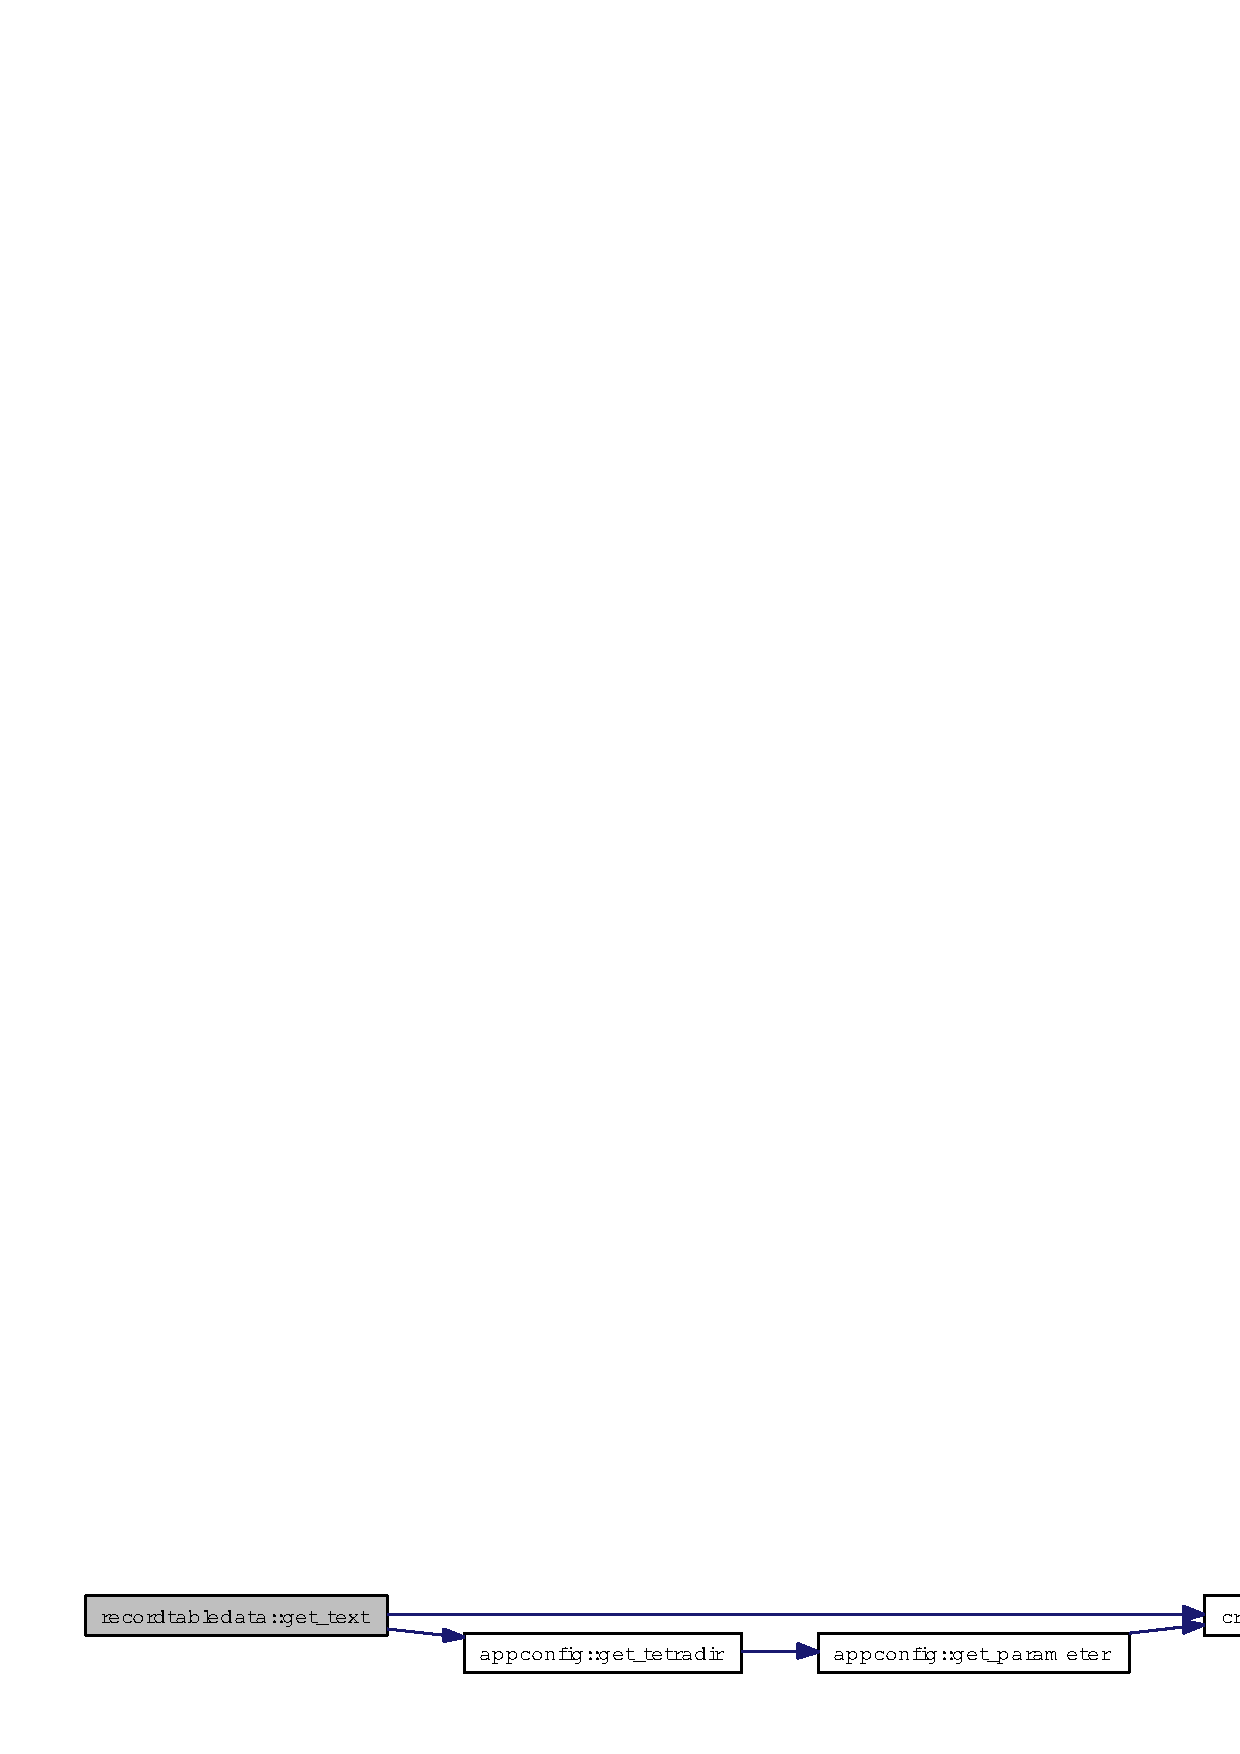
\includegraphics[width=331pt]{classrecordtabledata_2d91c0e1c41a40d2692e47fc2ca1fb78_cgraph}
\end{center}
\end{figure}


Here is the caller graph for this function:\begin{figure}[H]
\begin{center}
\leavevmode
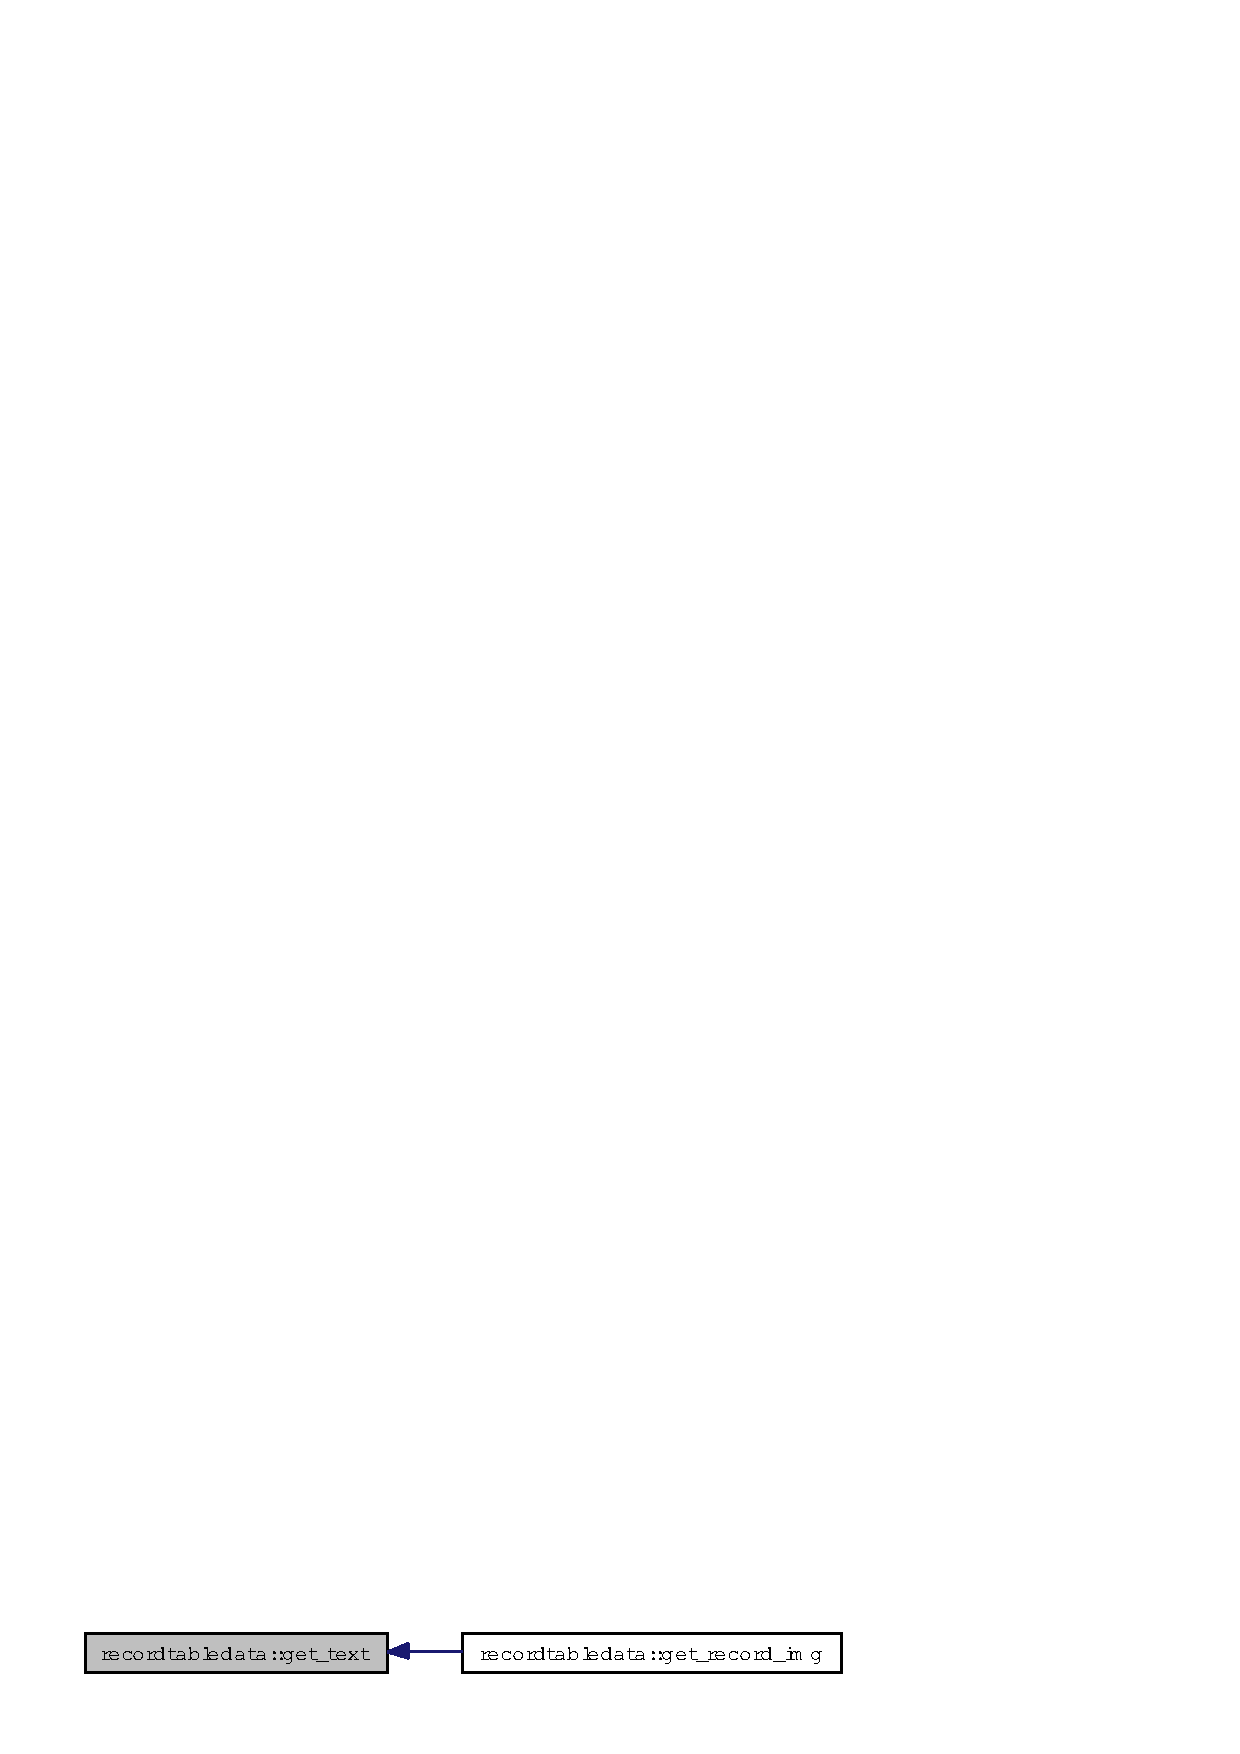
\includegraphics[width=204pt]{classrecordtabledata_2d91c0e1c41a40d2692e47fc2ca1fb78_icgraph}
\end{center}
\end{figure}
\index{recordtabledata@{recordtabledata}!get_field@{get\_\-field}}
\index{get_field@{get\_\-field}!recordtabledata@{recordtabledata}}
\subsubsection{\setlength{\rightskip}{0pt plus 5cm}QString recordtabledata::get\_\-field (QString {\em name}, int {\em pos}) const}\label{classrecordtabledata_1e5d2effed44a3b5c2072f570cf02594}




Definition at line 26 of file recordtabledata.cpp.

References critical\_\-error(), and table.

Referenced by recordtablemodel::data(), delete\_\-record(), recordtablescreen::edit\_\-field\_\-context(), and recordtablescreen::select().

Here is the call graph for this function:\begin{figure}[H]
\begin{center}
\leavevmode
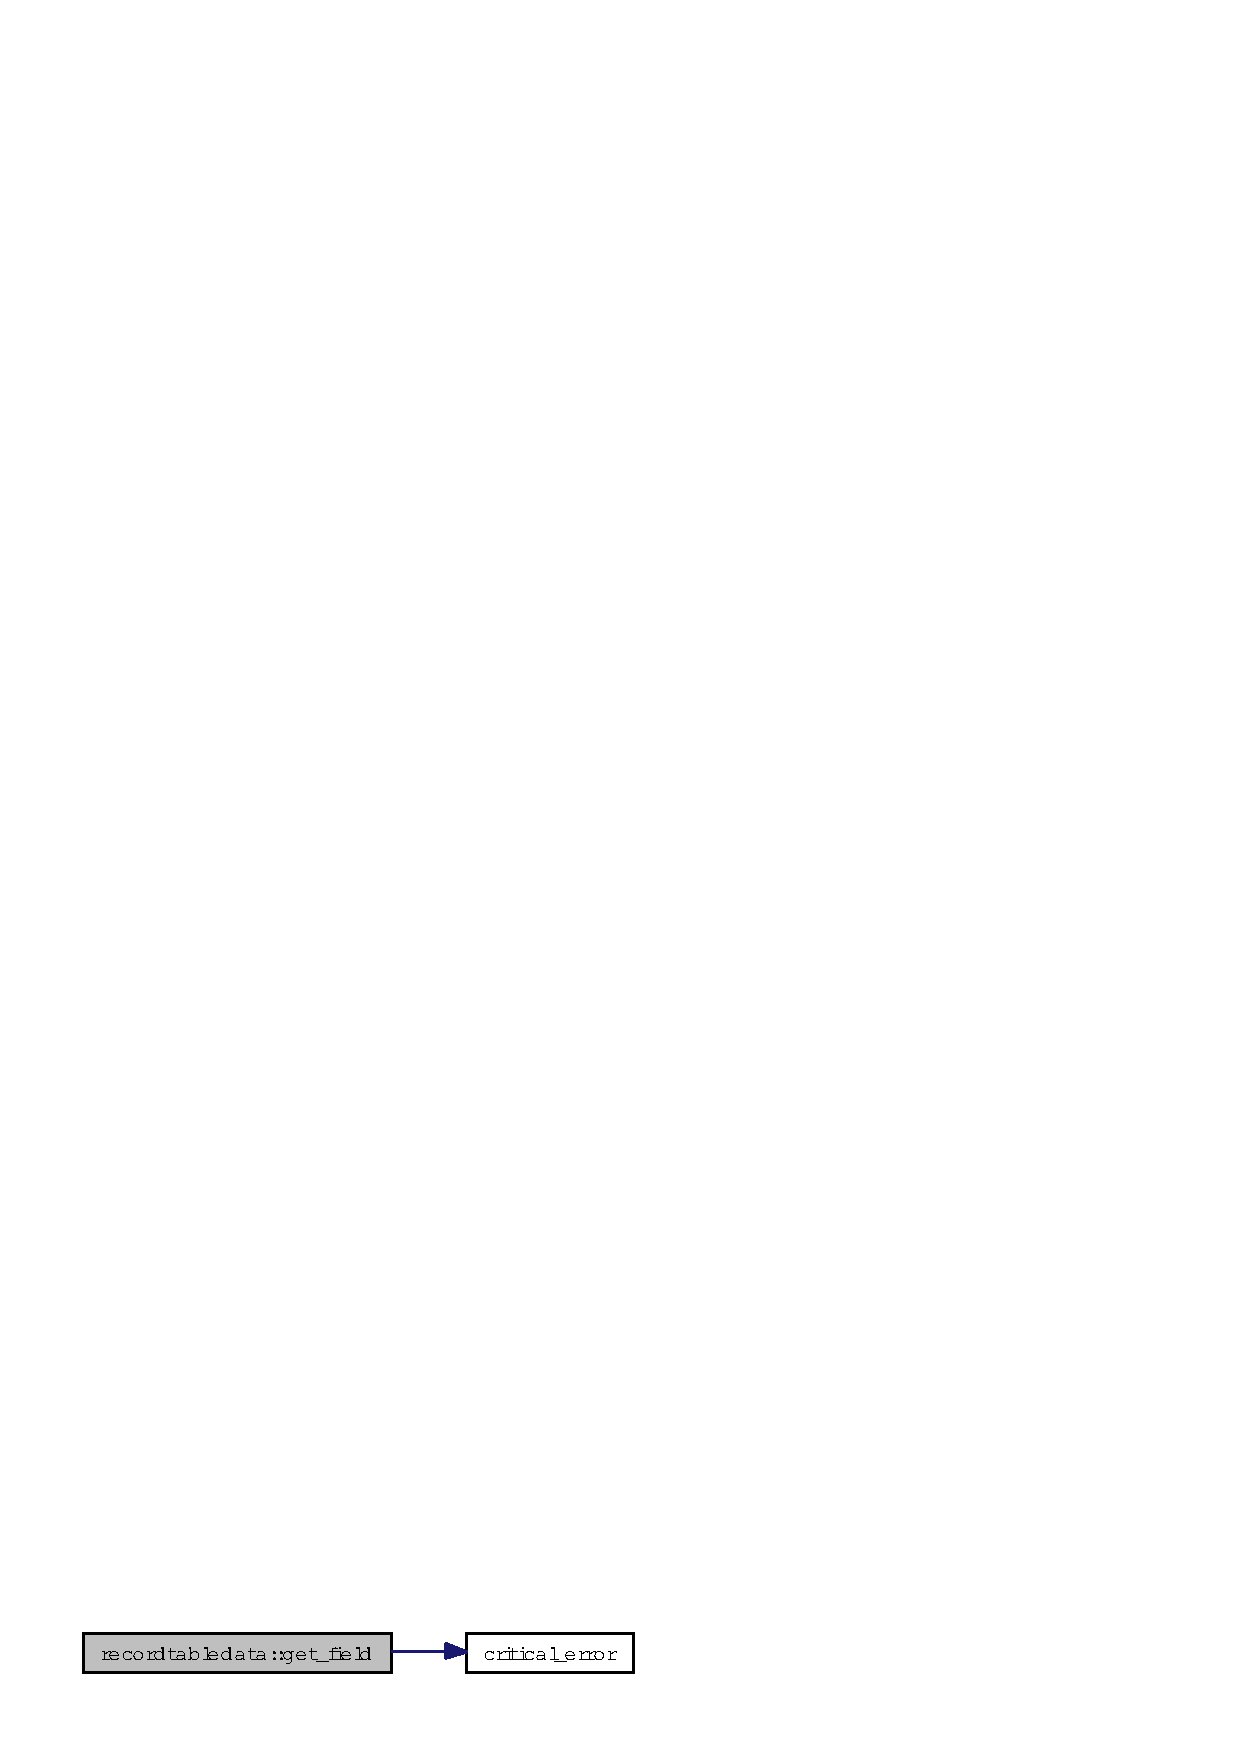
\includegraphics[width=154pt]{classrecordtabledata_1e5d2effed44a3b5c2072f570cf02594_cgraph}
\end{center}
\end{figure}


Here is the caller graph for this function:\begin{figure}[H]
\begin{center}
\leavevmode
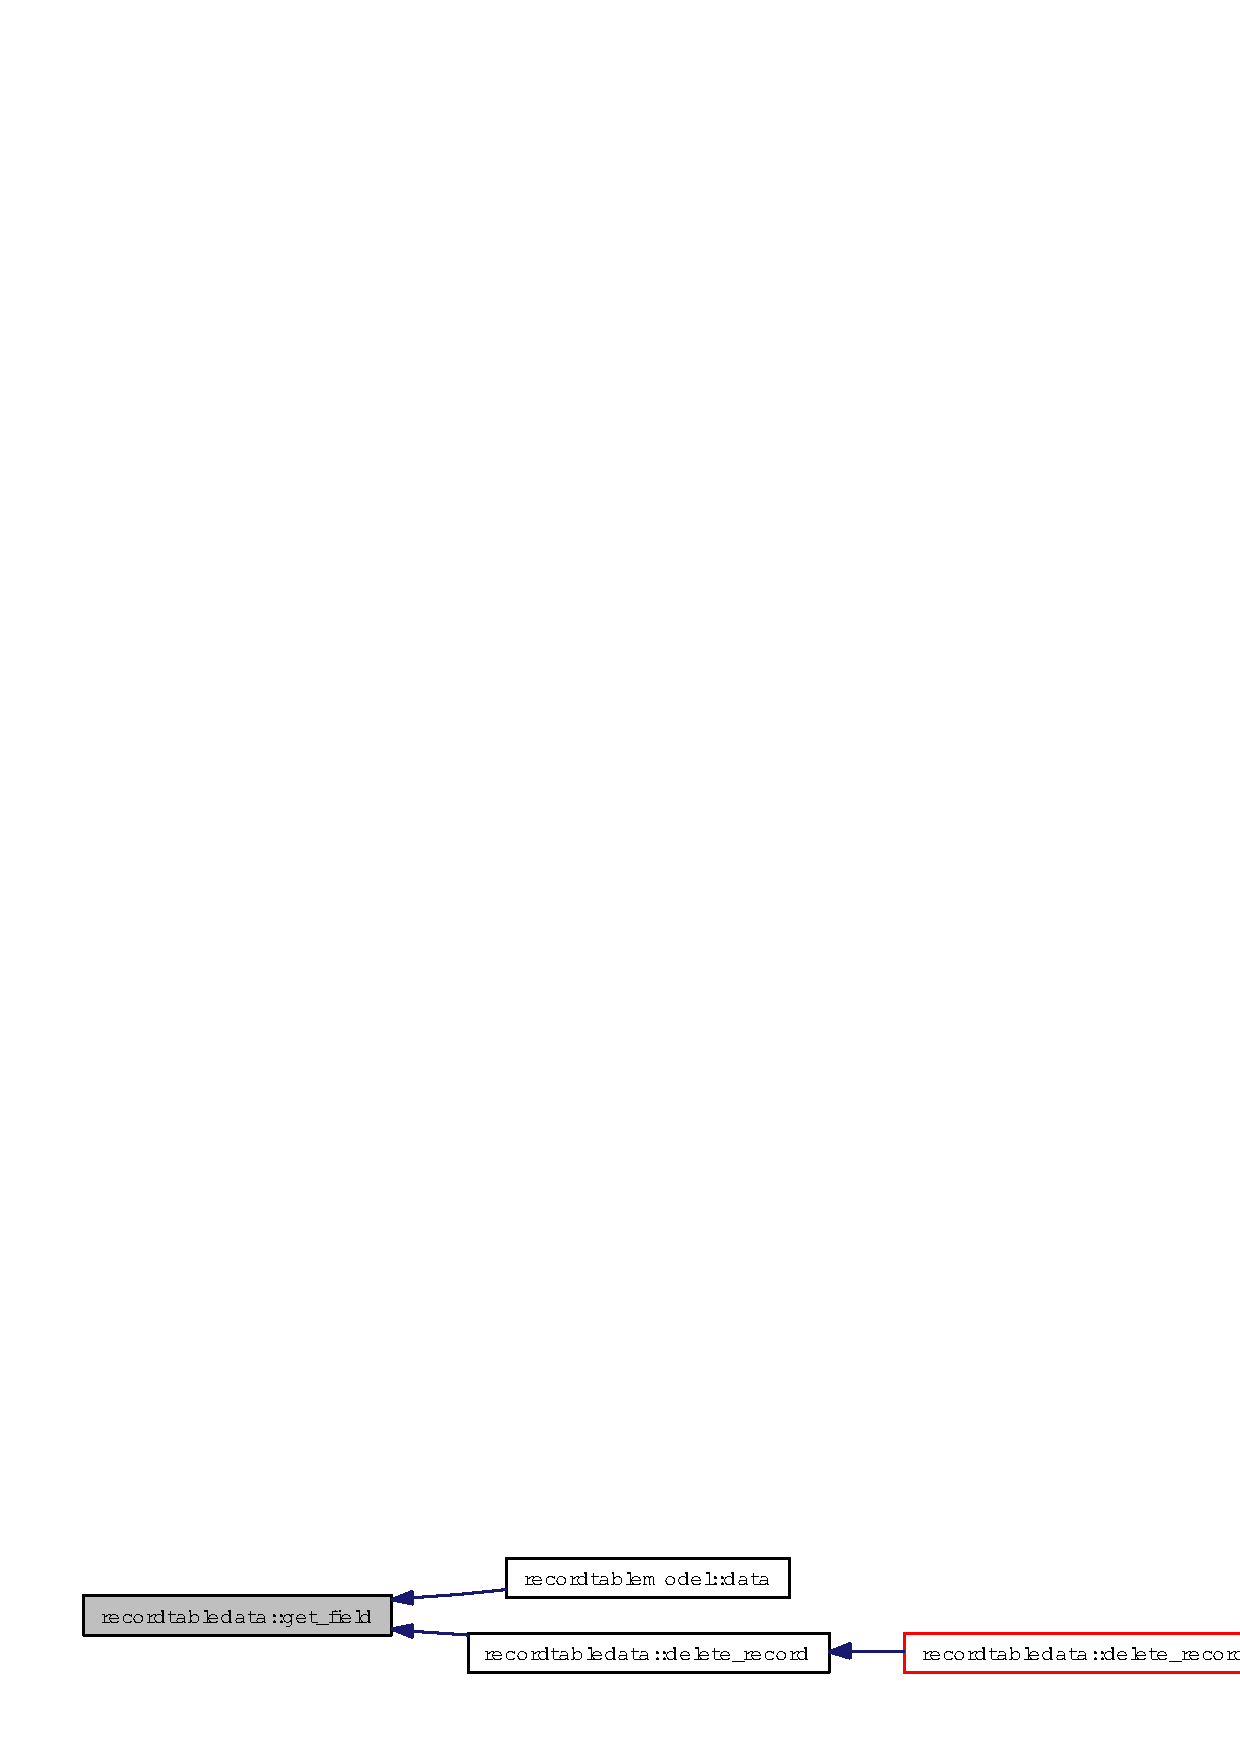
\includegraphics[width=308pt]{classrecordtabledata_1e5d2effed44a3b5c2072f570cf02594_icgraph}
\end{center}
\end{figure}
\index{recordtabledata@{recordtabledata}!set_field@{set\_\-field}}
\index{set_field@{set\_\-field}!recordtabledata@{recordtabledata}}
\subsubsection{\setlength{\rightskip}{0pt plus 5cm}void recordtabledata::set\_\-field (QString {\em name}, QString {\em value}, int {\em pos})}\label{classrecordtabledata_700883543df1f758a8d9b6ceb69a98be}




Definition at line 50 of file recordtabledata.cpp.

References critical\_\-error(), and table.

Referenced by recordtablemodel::set\-Data().

Here is the call graph for this function:\begin{figure}[H]
\begin{center}
\leavevmode
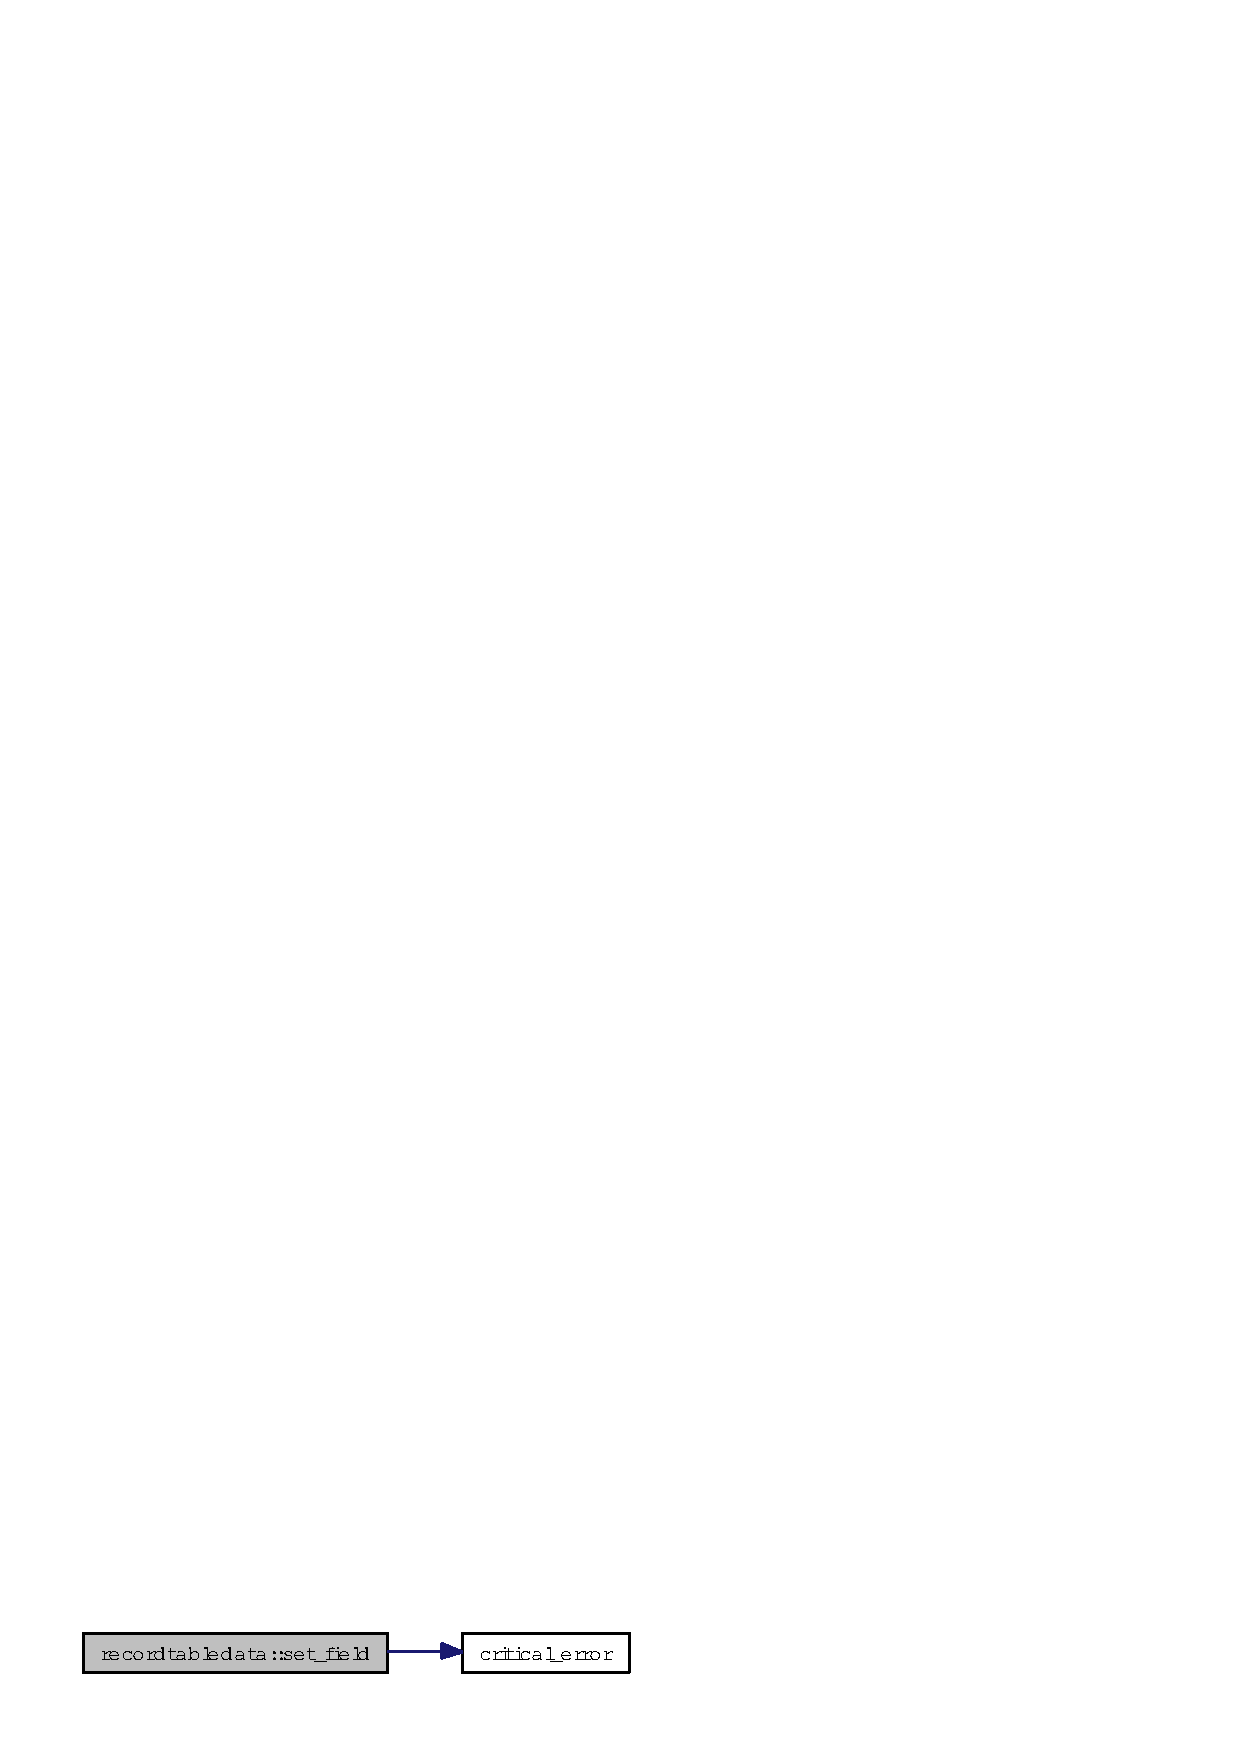
\includegraphics[width=153pt]{classrecordtabledata_700883543df1f758a8d9b6ceb69a98be_cgraph}
\end{center}
\end{figure}


Here is the caller graph for this function:\begin{figure}[H]
\begin{center}
\leavevmode
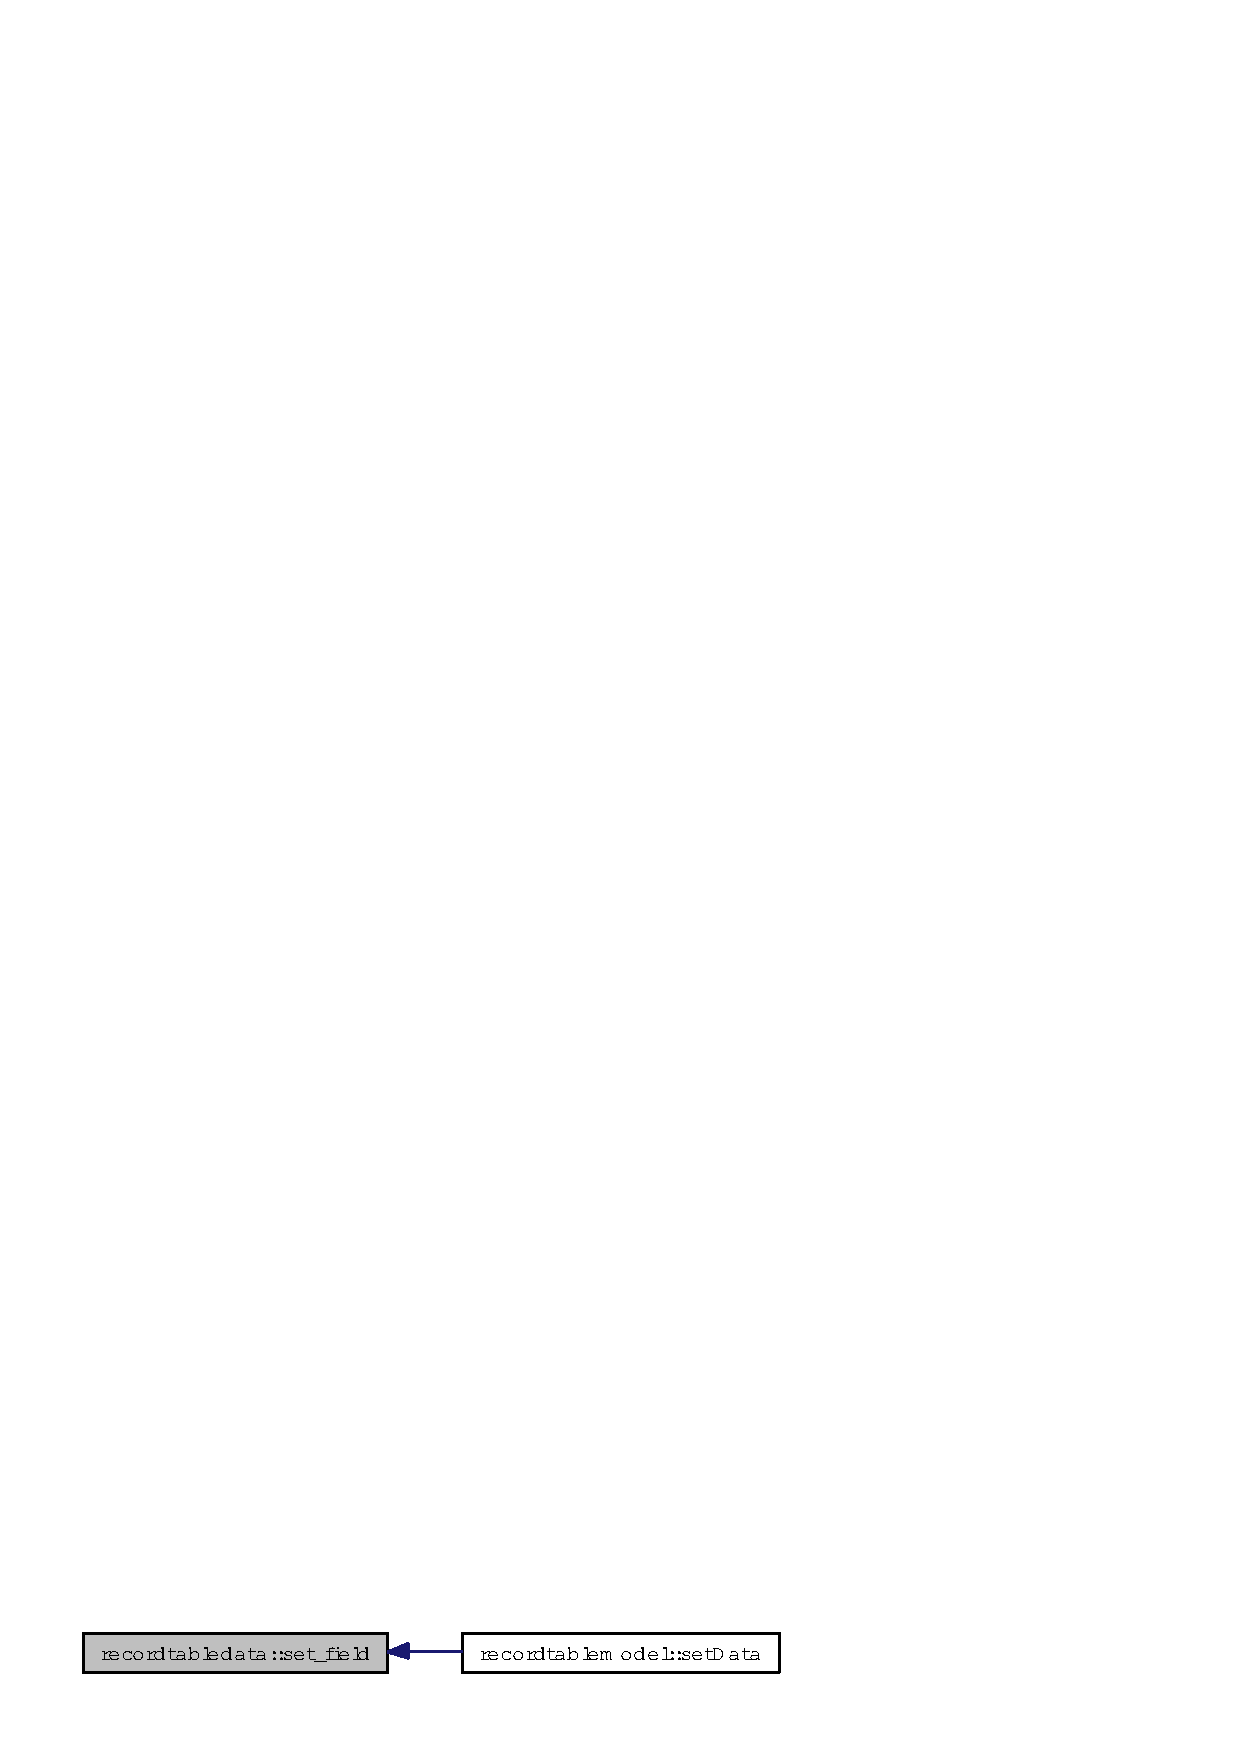
\includegraphics[width=189pt]{classrecordtabledata_700883543df1f758a8d9b6ceb69a98be_icgraph}
\end{center}
\end{figure}
\index{recordtabledata@{recordtabledata}!get_fields@{get\_\-fields}}
\index{get_fields@{get\_\-fields}!recordtabledata@{recordtabledata}}
\subsubsection{\setlength{\rightskip}{0pt plus 5cm}QMap$<$ QString, QString $>$ recordtabledata::get\_\-fields (int {\em pos}) const}\label{classrecordtabledata_bb59c7c87809612f261d087b3ea14d94}




Definition at line 94 of file recordtabledata.cpp.

References critical\_\-error(), and table.

Referenced by get\_\-record\_\-img().

Here is the call graph for this function:\begin{figure}[H]
\begin{center}
\leavevmode
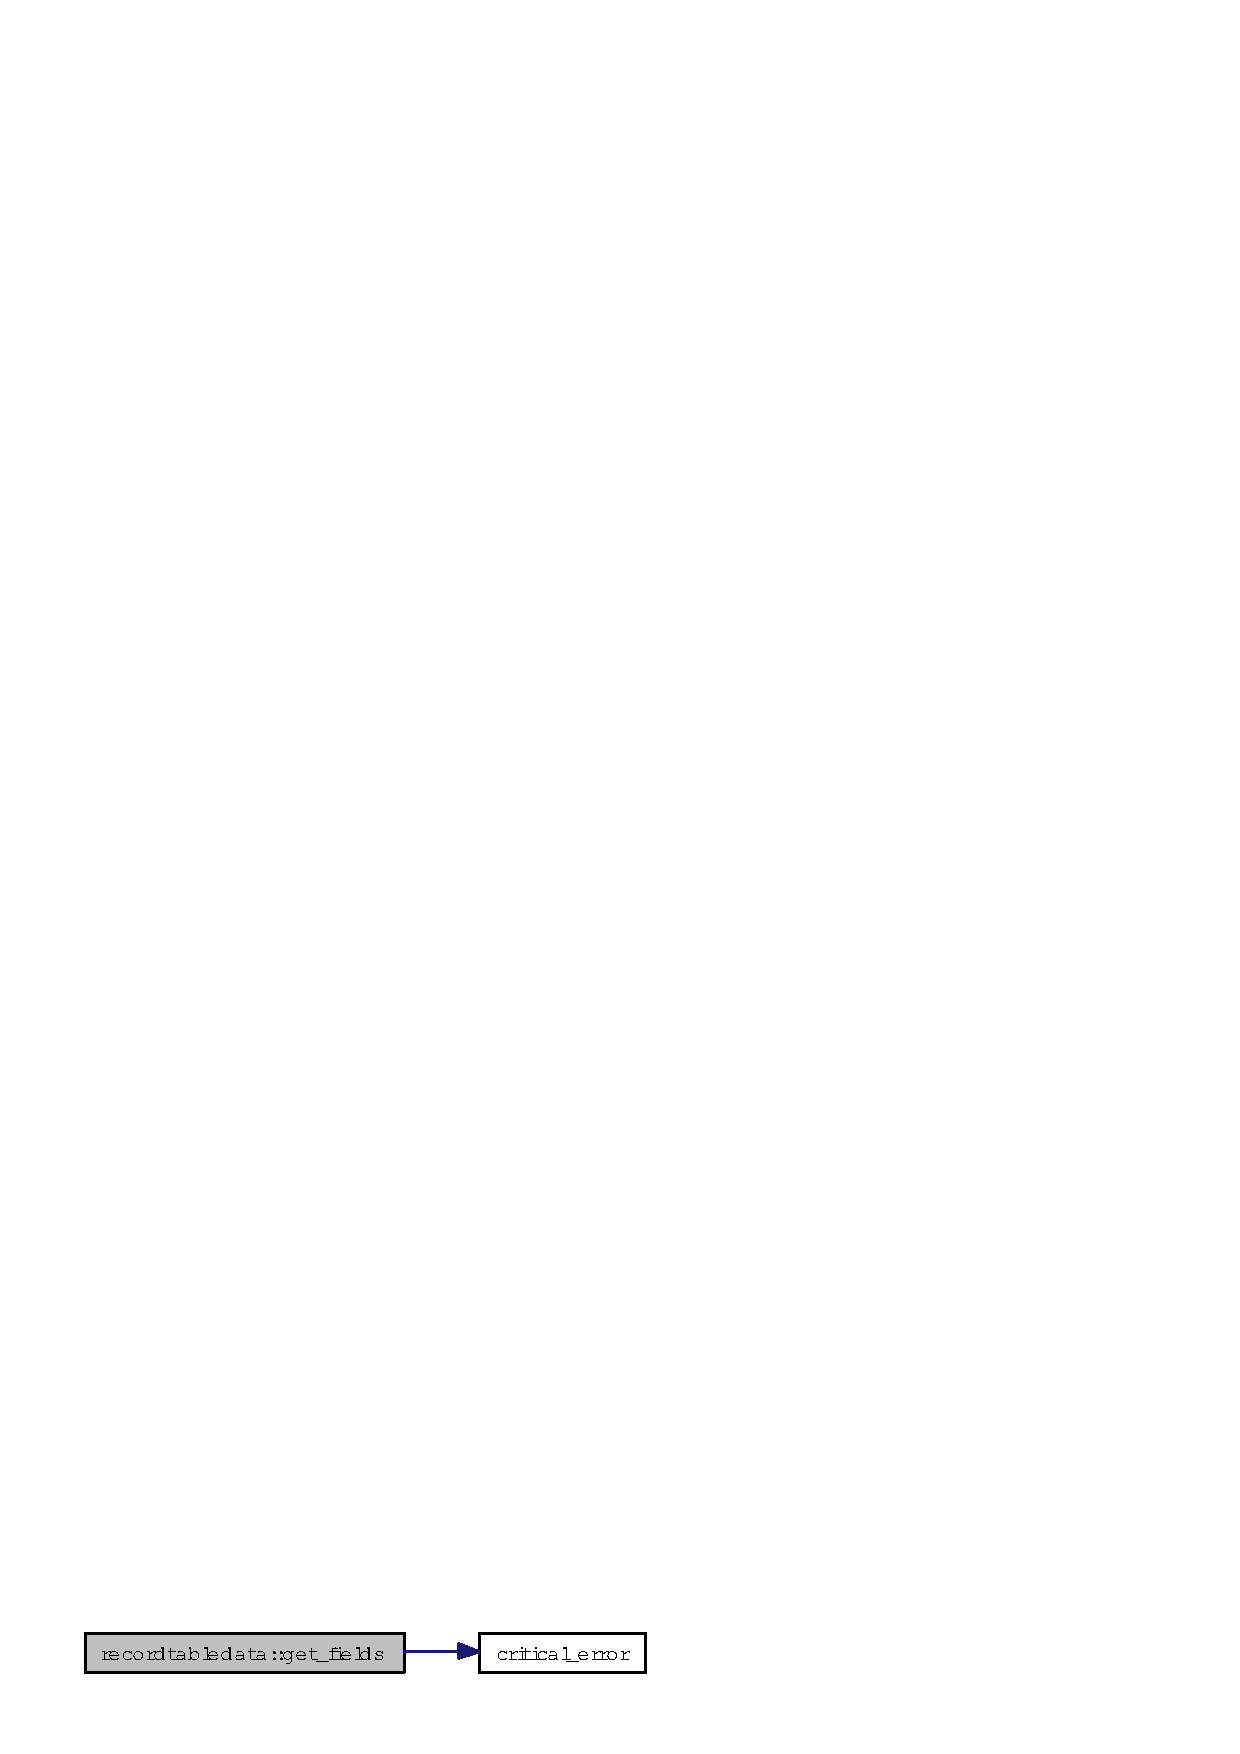
\includegraphics[width=157pt]{classrecordtabledata_bb59c7c87809612f261d087b3ea14d94_cgraph}
\end{center}
\end{figure}


Here is the caller graph for this function:\begin{figure}[H]
\begin{center}
\leavevmode
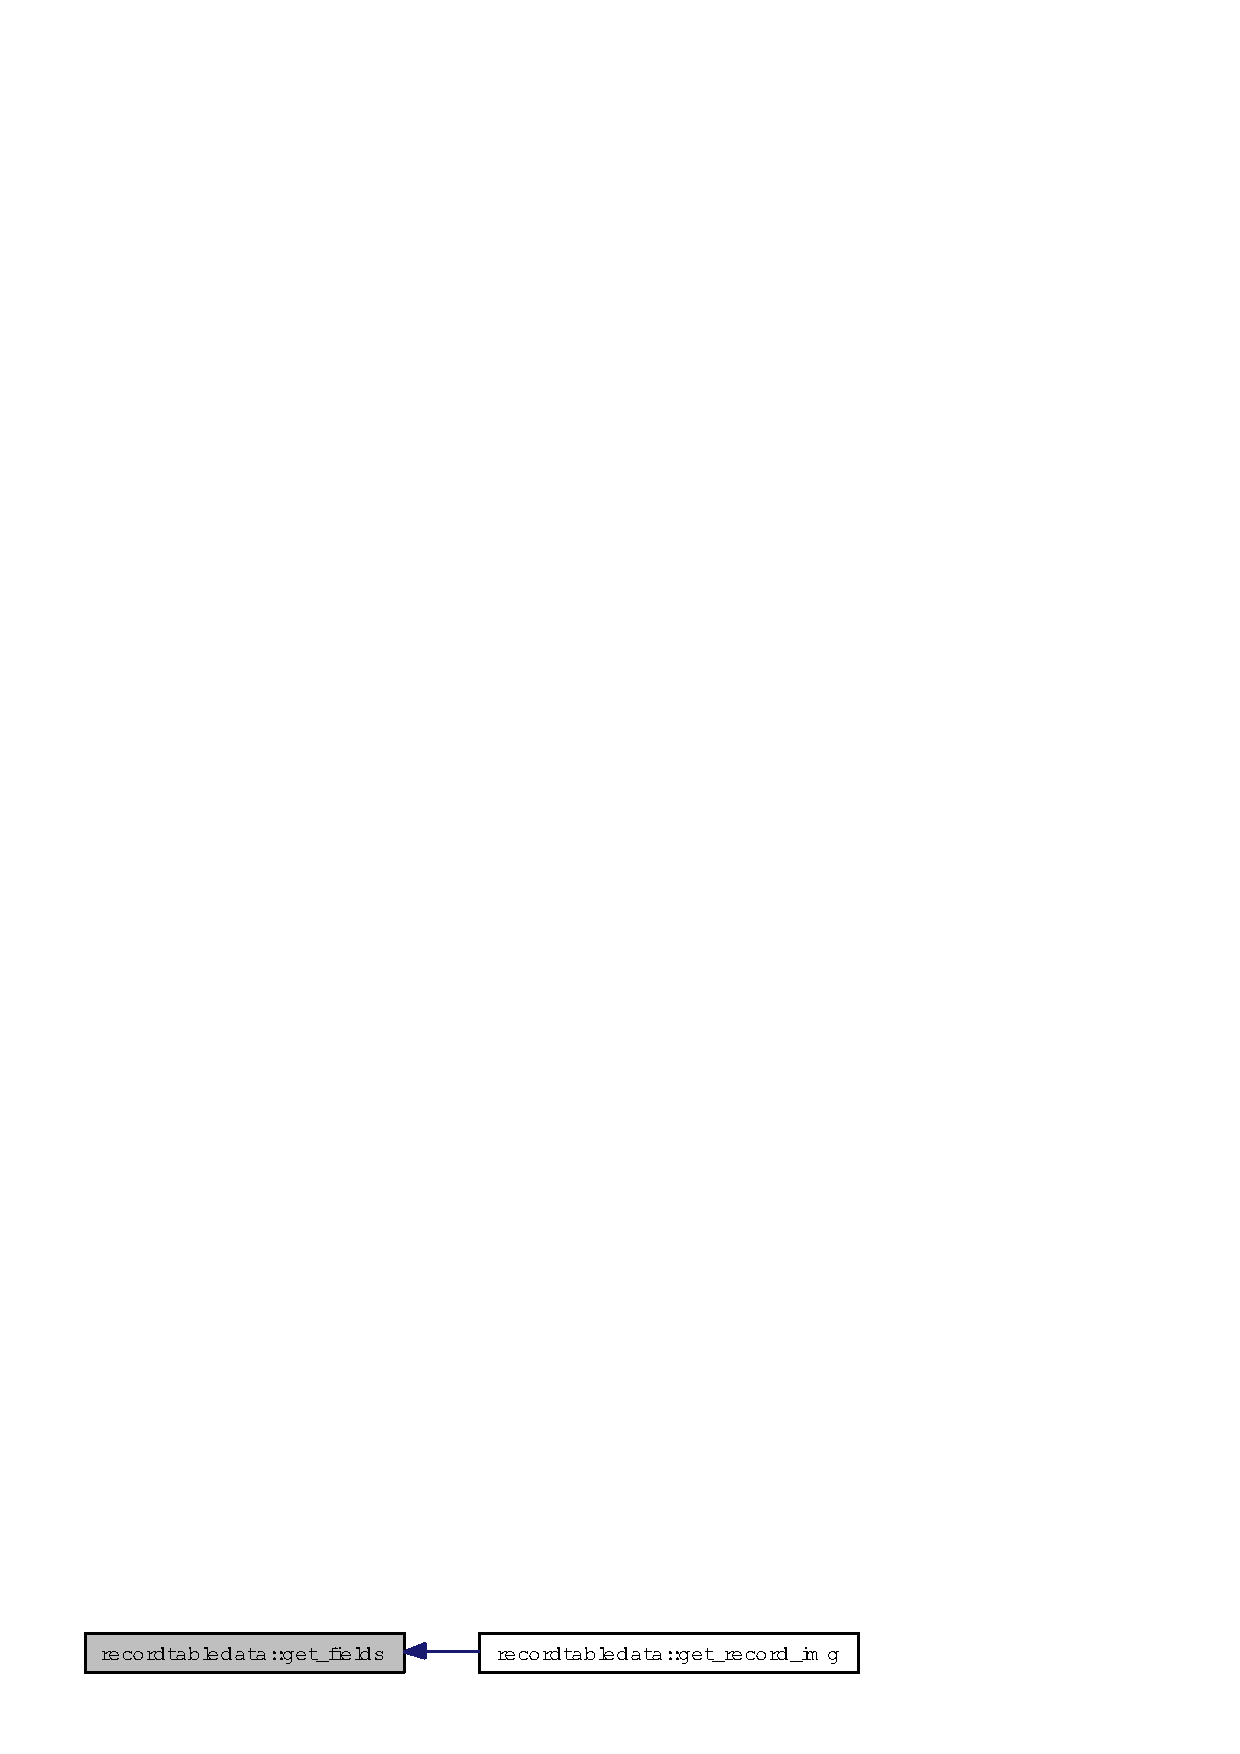
\includegraphics[width=208pt]{classrecordtabledata_bb59c7c87809612f261d087b3ea14d94_icgraph}
\end{center}
\end{figure}
\index{recordtabledata@{recordtabledata}!get_record_img@{get\_\-record\_\-img}}
\index{get_record_img@{get\_\-record\_\-img}!recordtabledata@{recordtabledata}}
\subsubsection{\setlength{\rightskip}{0pt plus 5cm}QMap$<$ QString, QString $>$ recordtabledata::get\_\-record\_\-img (int {\em pos}) const}\label{classrecordtabledata_8483238f577c62c4d3a8467acda1636d}




Definition at line 128 of file recordtabledata.cpp.

References get\_\-fields(), get\_\-text(), and table.

Referenced by recordtablescreen::copy().

Here is the call graph for this function:\begin{figure}[H]
\begin{center}
\leavevmode
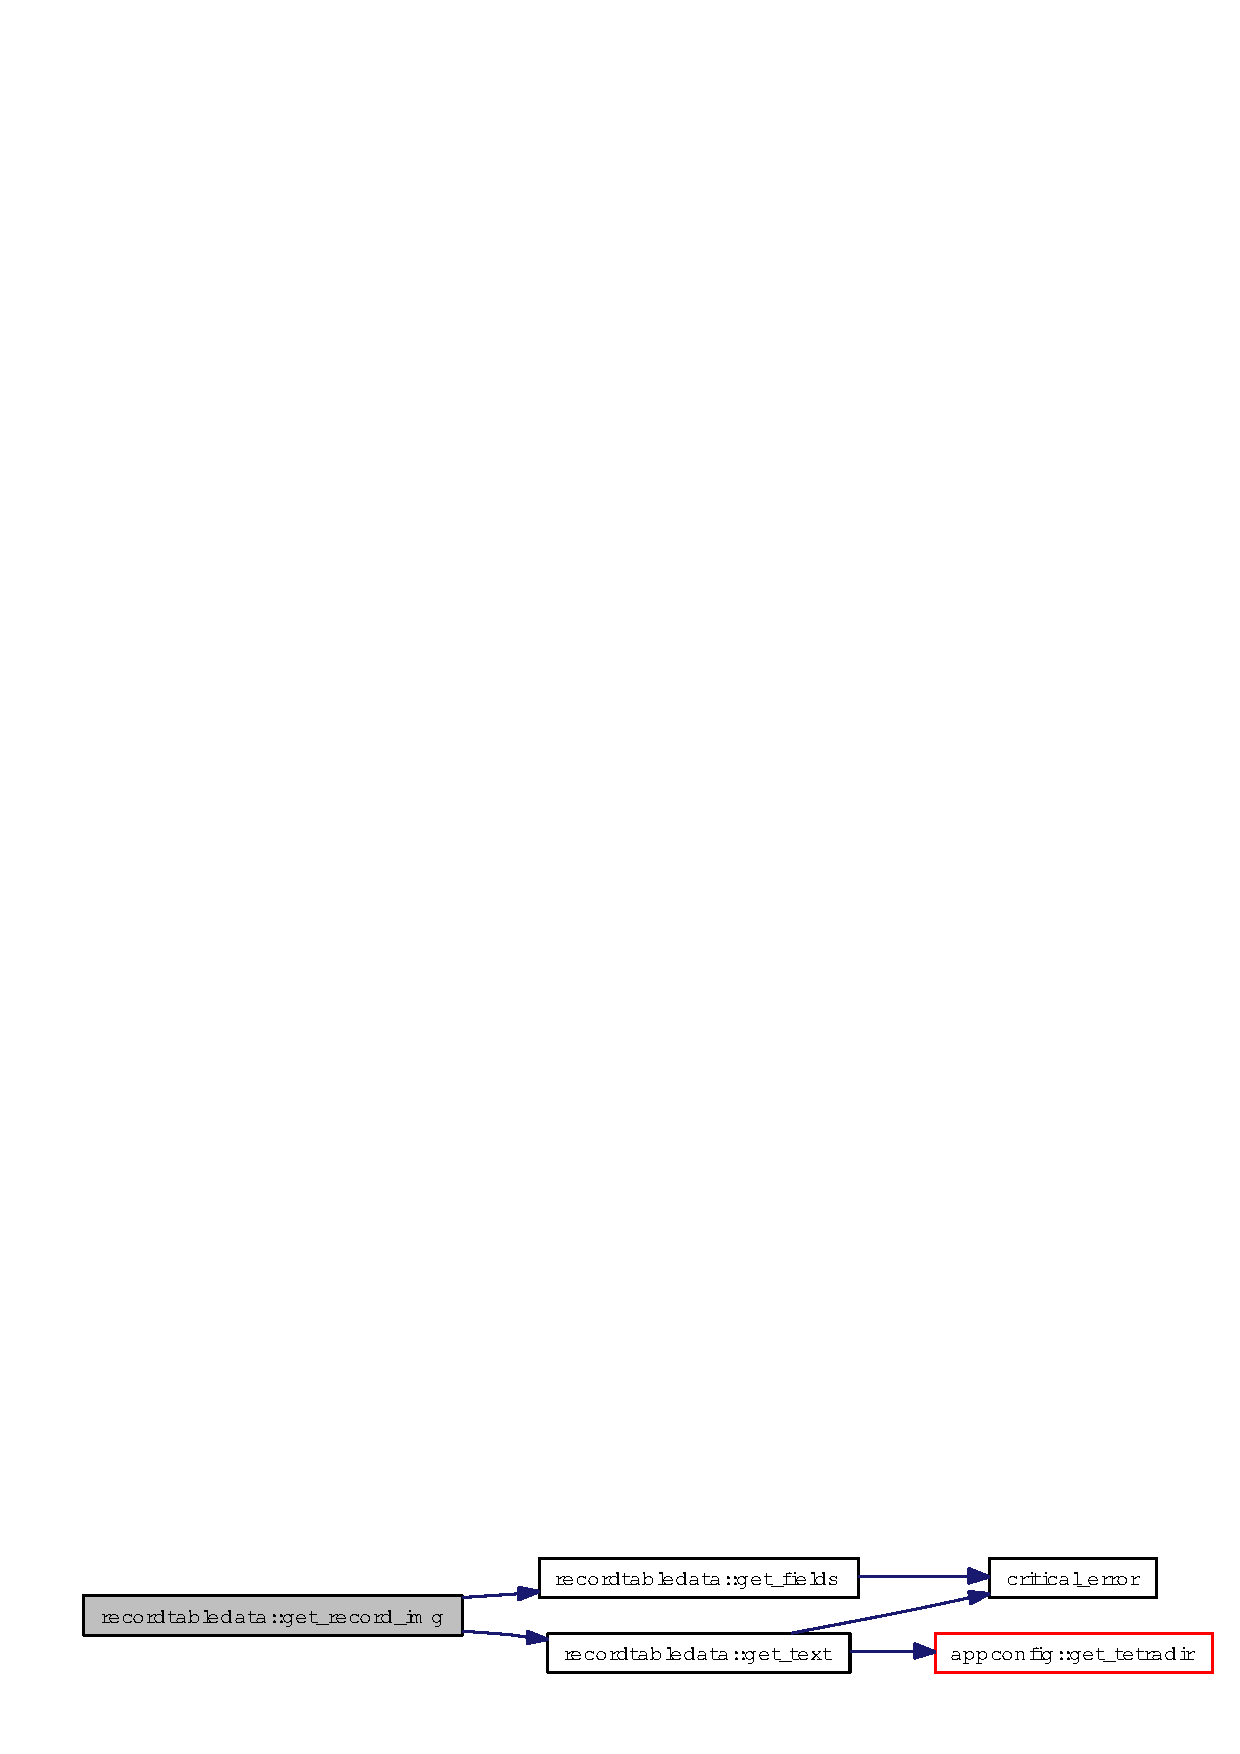
\includegraphics[width=293pt]{classrecordtabledata_8483238f577c62c4d3a8467acda1636d_cgraph}
\end{center}
\end{figure}
\index{recordtabledata@{recordtabledata}!init@{init}}
\index{init@{init}!recordtabledata@{recordtabledata}}
\subsubsection{\setlength{\rightskip}{0pt plus 5cm}void recordtabledata::init (QDom\-Element {\em dommodel})}\label{classrecordtabledata_c8a0b71ad80fbdd4559b9dfe8c6520b3}




Definition at line 144 of file recordtabledata.cpp.

References setup\_\-data\_\-from\_\-dom().

Referenced by Tree\-Item::recordtable\_\-init().

Here is the call graph for this function:\begin{figure}[H]
\begin{center}
\leavevmode
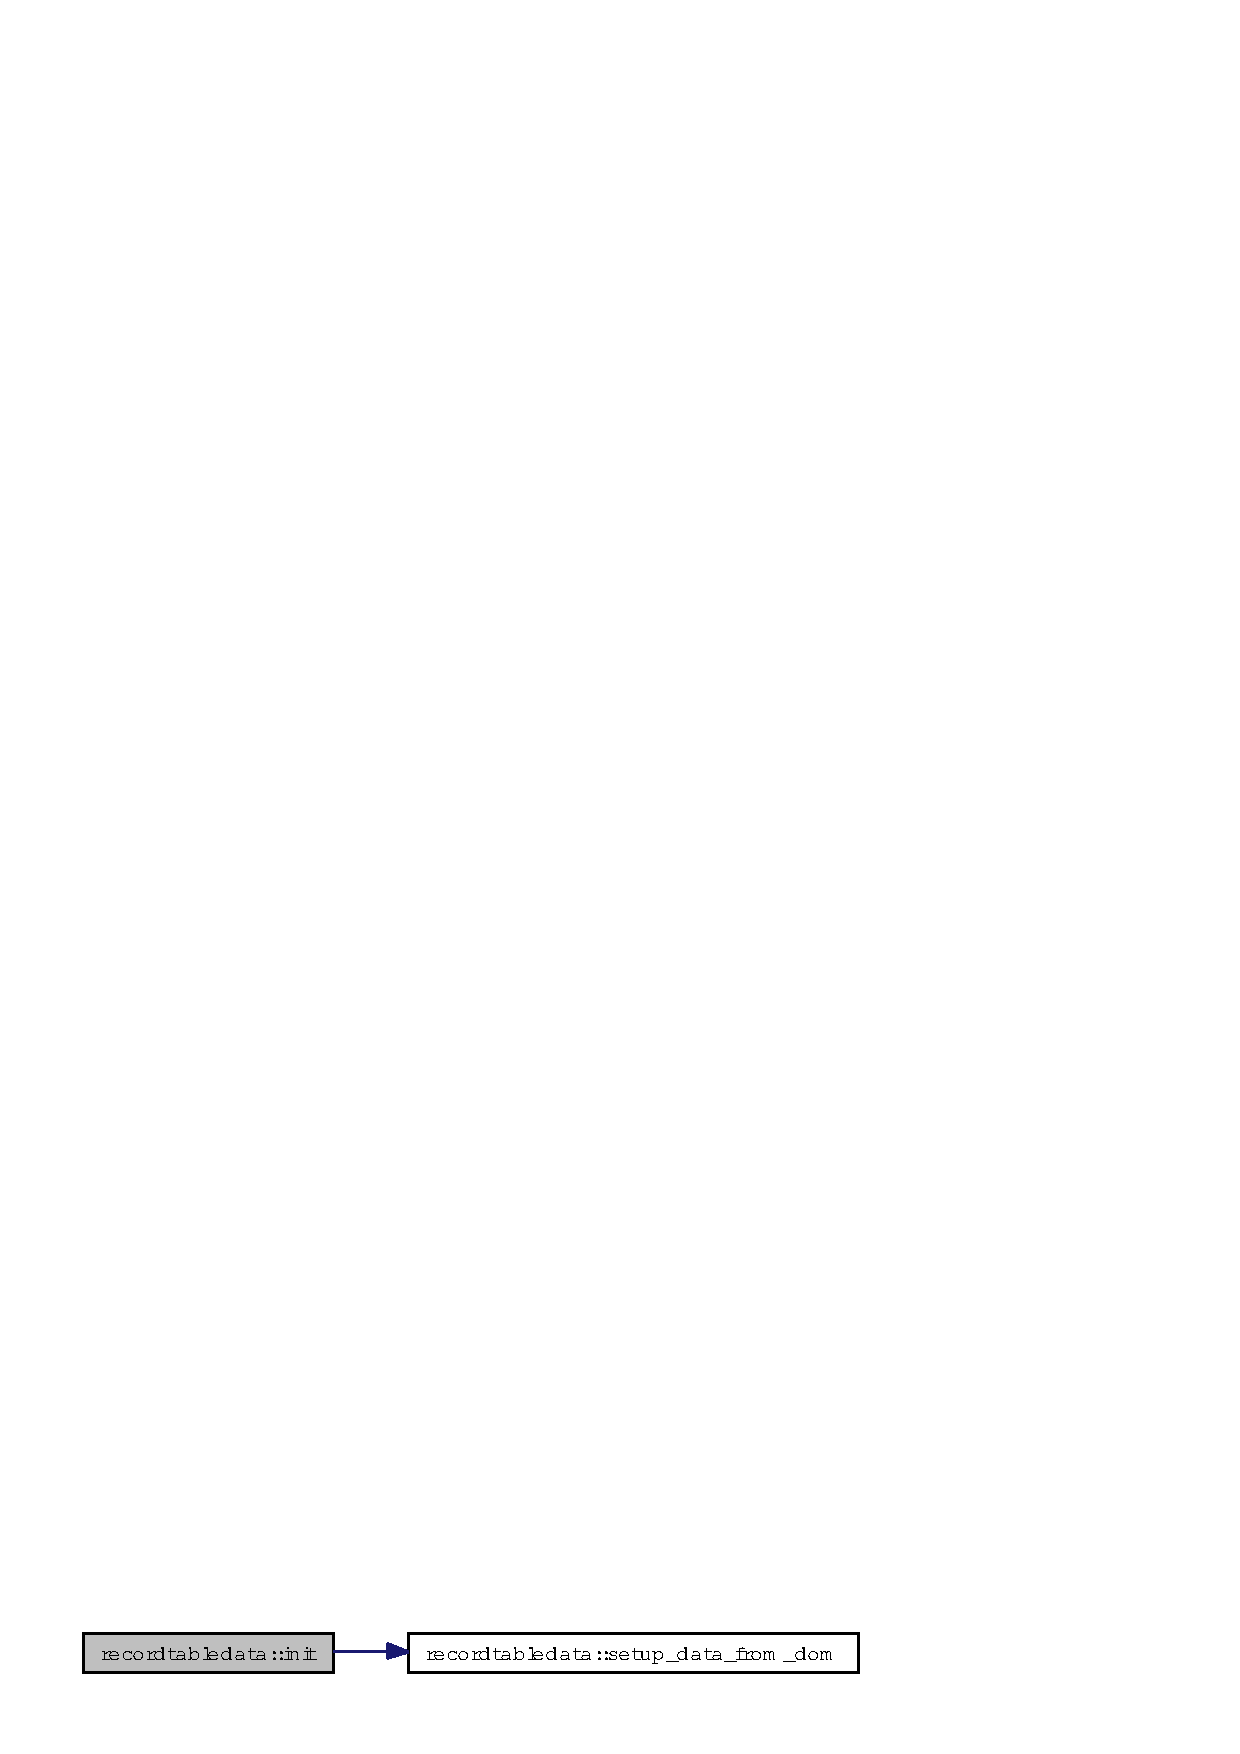
\includegraphics[width=208pt]{classrecordtabledata_c8a0b71ad80fbdd4559b9dfe8c6520b3_cgraph}
\end{center}
\end{figure}


Here is the caller graph for this function:\begin{figure}[H]
\begin{center}
\leavevmode
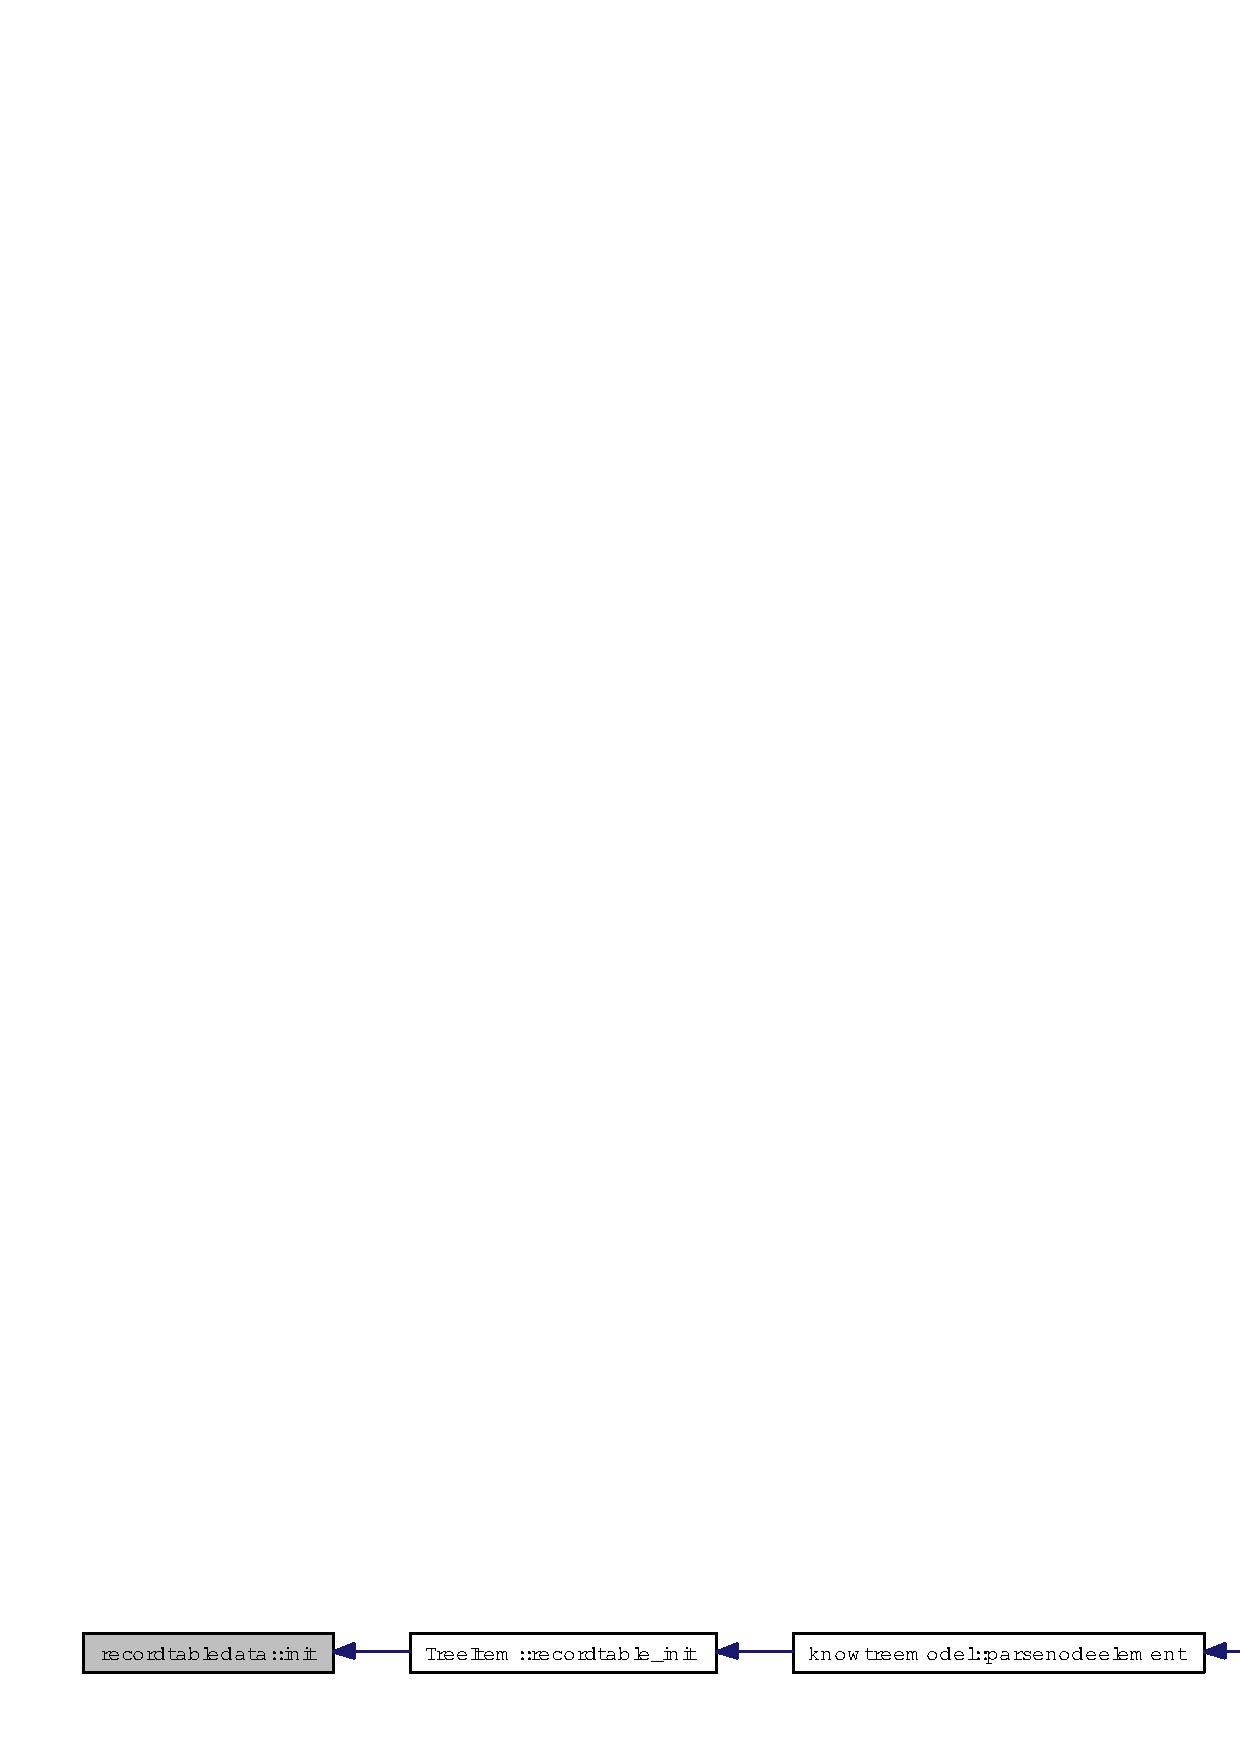
\includegraphics[width=402pt]{classrecordtabledata_c8a0b71ad80fbdd4559b9dfe8c6520b3_icgraph}
\end{center}
\end{figure}
\index{recordtabledata@{recordtabledata}!clear@{clear}}
\index{clear@{clear}!recordtabledata@{recordtabledata}}
\subsubsection{\setlength{\rightskip}{0pt plus 5cm}void recordtabledata::clear (void)}\label{classrecordtabledata_64bf565f5a8ef057d92db05b8478c4fe}




Definition at line 414 of file recordtabledata.cpp.

References delete\_\-records(), and table.

Referenced by Tree\-Item::recordtable\_\-clear().

Here is the call graph for this function:\begin{figure}[H]
\begin{center}
\leavevmode
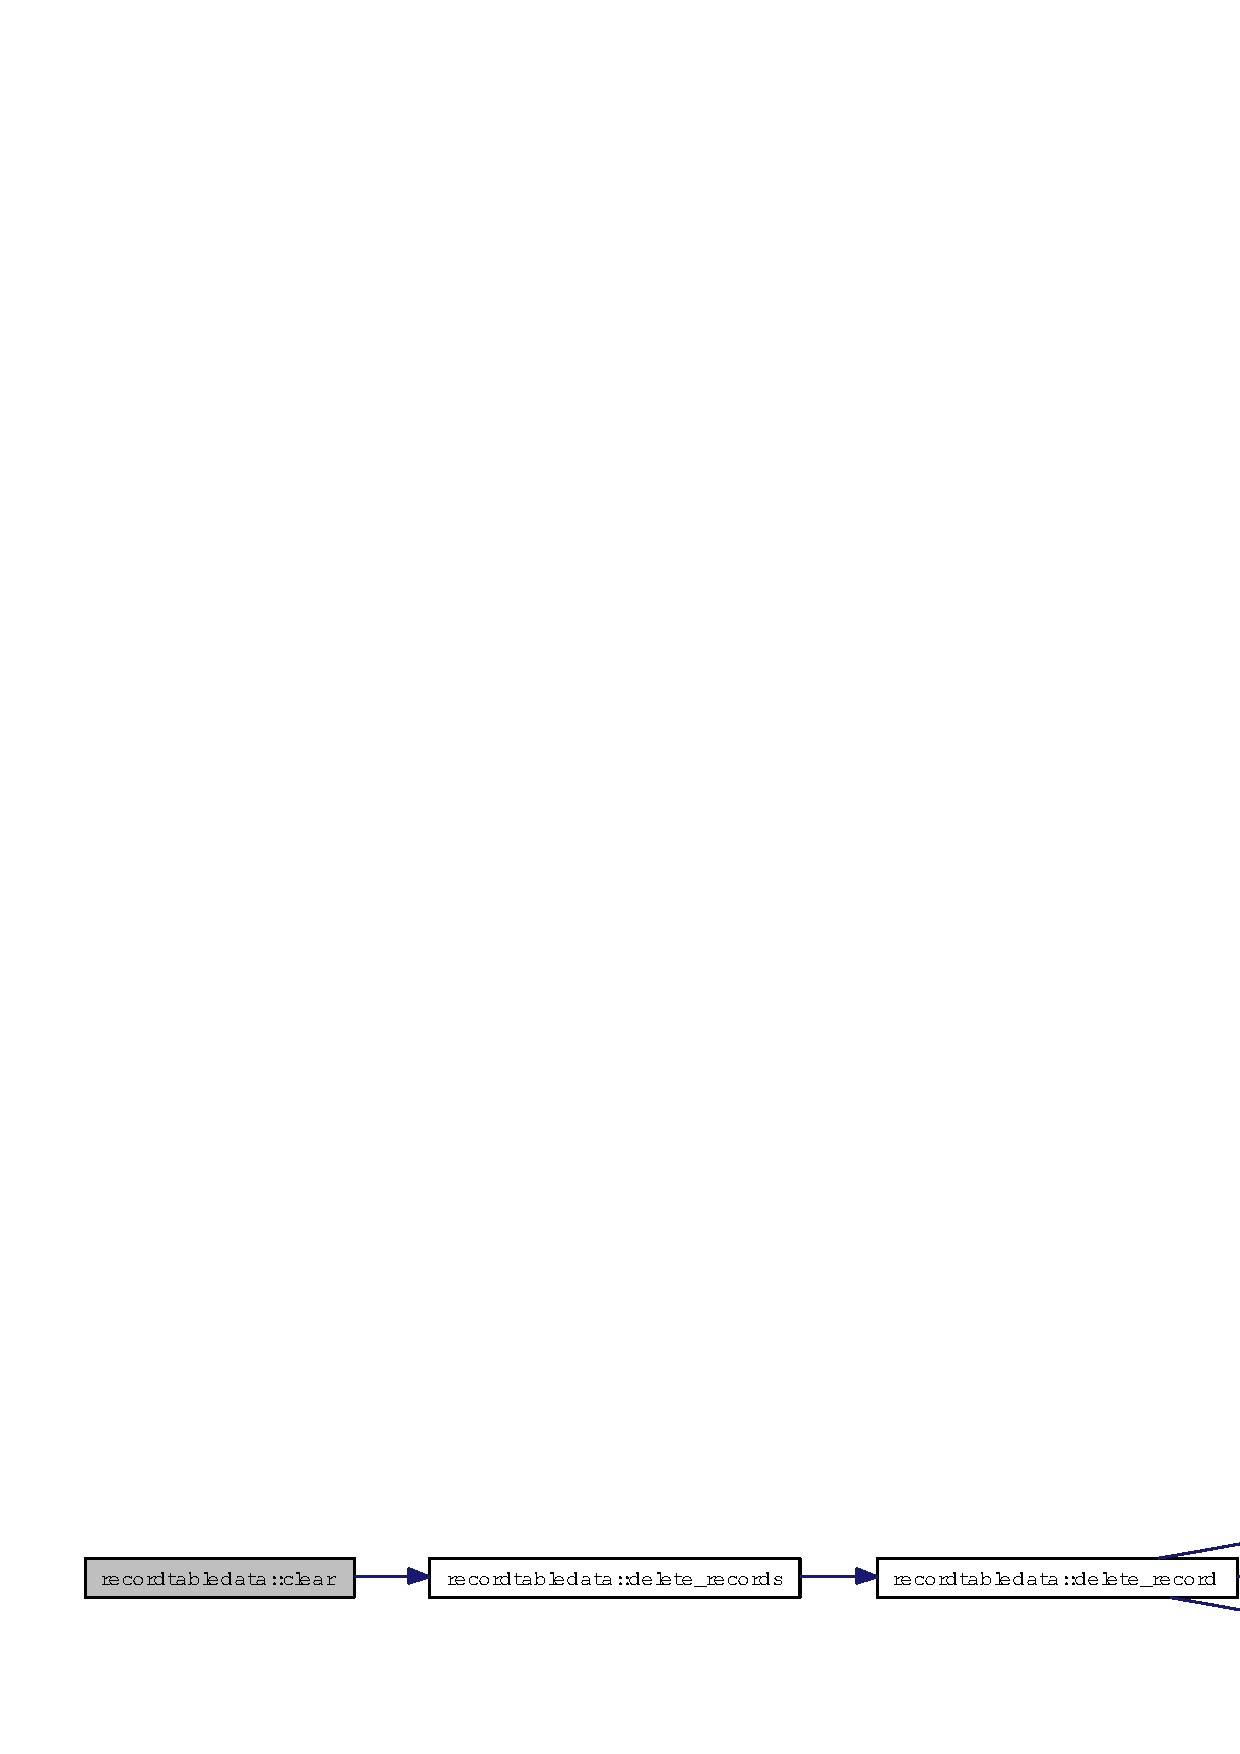
\includegraphics[width=391pt]{classrecordtabledata_64bf565f5a8ef057d92db05b8478c4fe_cgraph}
\end{center}
\end{figure}


Here is the caller graph for this function:\begin{figure}[H]
\begin{center}
\leavevmode
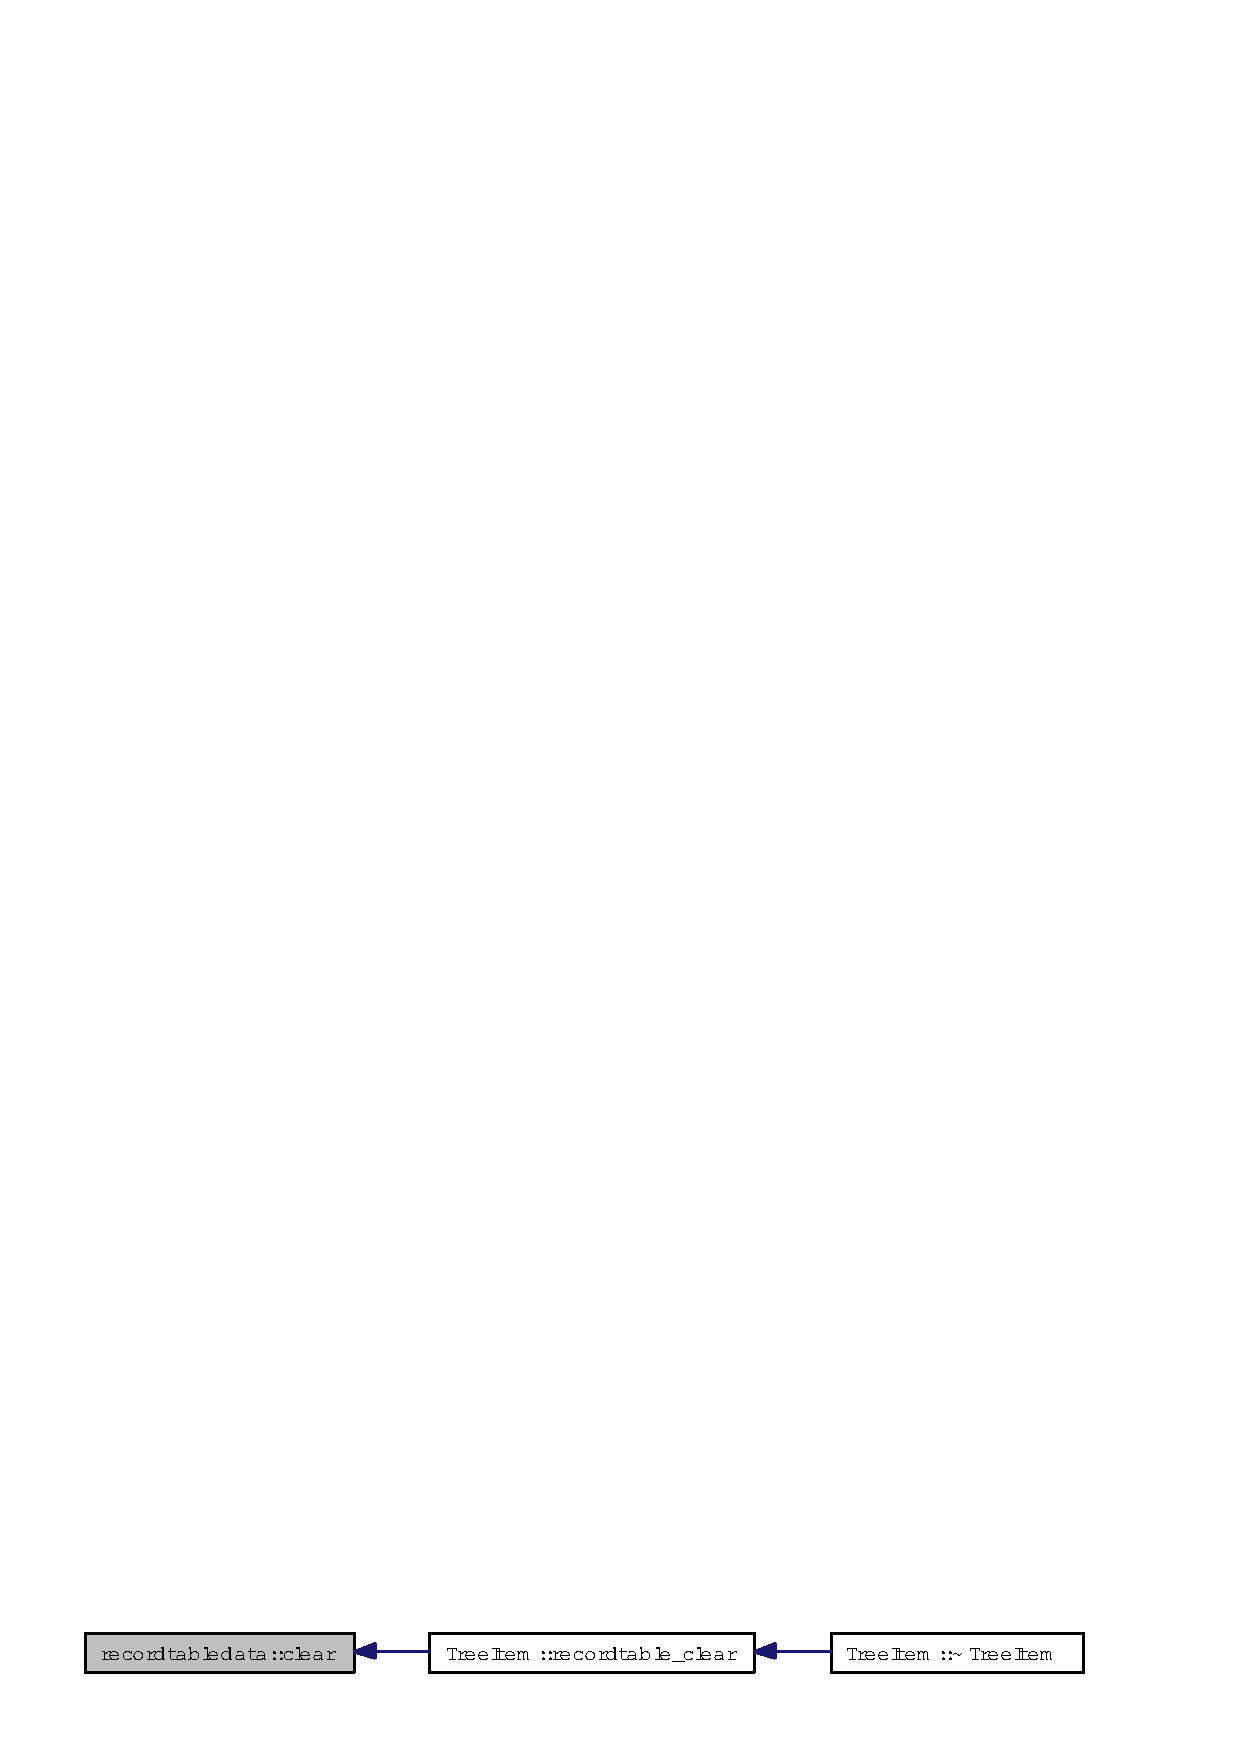
\includegraphics[width=262pt]{classrecordtabledata_64bf565f5a8ef057d92db05b8478c4fe_icgraph}
\end{center}
\end{figure}
\index{recordtabledata@{recordtabledata}!size@{size}}
\index{size@{size}!recordtabledata@{recordtabledata}}
\subsubsection{\setlength{\rightskip}{0pt plus 5cm}int recordtabledata::size (void)}\label{classrecordtabledata_550a266ba595511d23216feb085853a9}




Definition at line 425 of file recordtabledata.cpp.

References table.

Referenced by recordtablescreen::delete\_\-records(), Tree\-Item::recordtable\_\-getrowcount(), and recordtablemodel::row\-Count().

Here is the caller graph for this function:\begin{figure}[H]
\begin{center}
\leavevmode
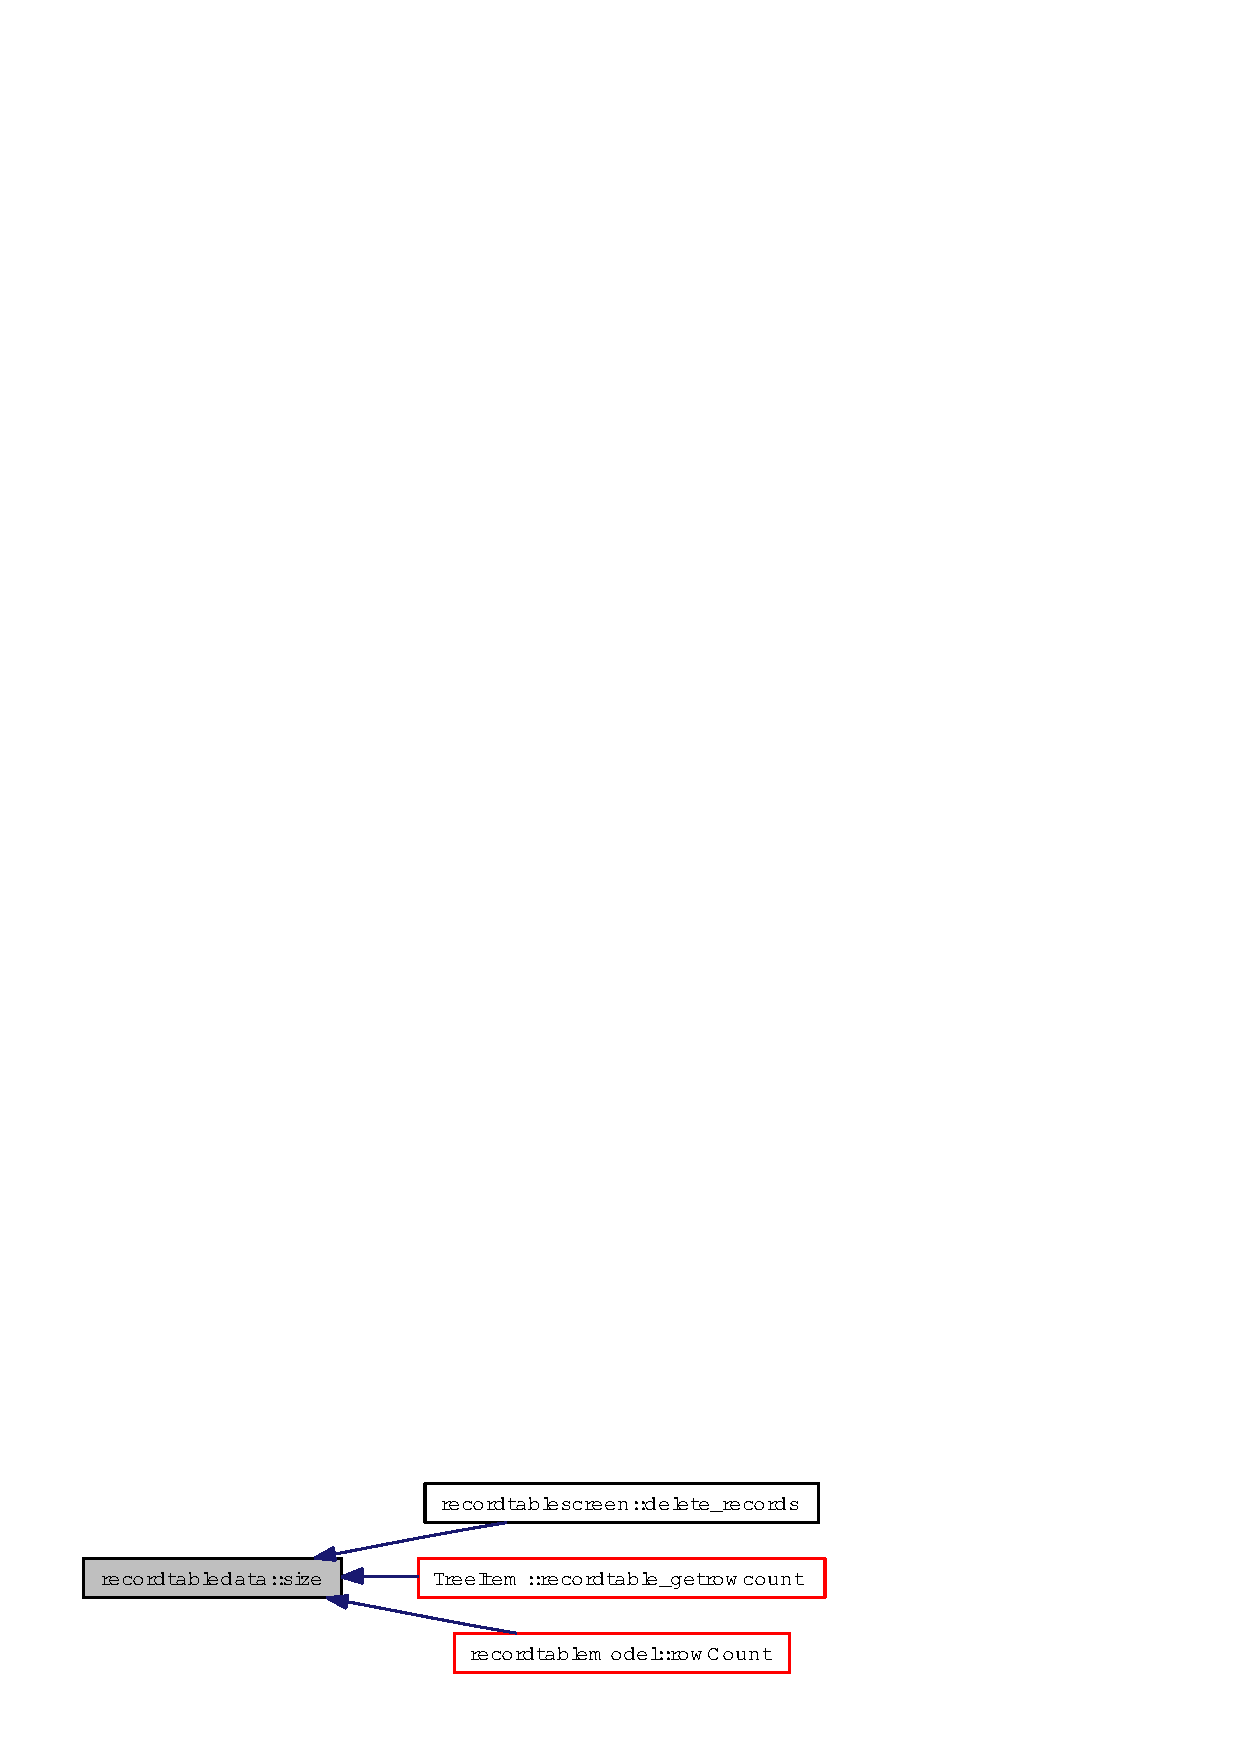
\includegraphics[width=200pt]{classrecordtabledata_550a266ba595511d23216feb085853a9_icgraph}
\end{center}
\end{figure}
\index{recordtabledata@{recordtabledata}!export_data_to_dom@{export\_\-data\_\-to\_\-dom}}
\index{export_data_to_dom@{export\_\-data\_\-to\_\-dom}!recordtabledata@{recordtabledata}}
\subsubsection{\setlength{\rightskip}{0pt plus 5cm}QDom\-Document recordtabledata::export\_\-data\_\-to\_\-dom (void)}\label{classrecordtabledata_fd04b0ca1500e0fd9ac3fb2d56c12b82}




Definition at line 208 of file recordtabledata.cpp.

References table.

Referenced by Tree\-Item::recordtable\_\-export\_\-data\_\-to\_\-dom().

Here is the caller graph for this function:\begin{figure}[H]
\begin{center}
\leavevmode
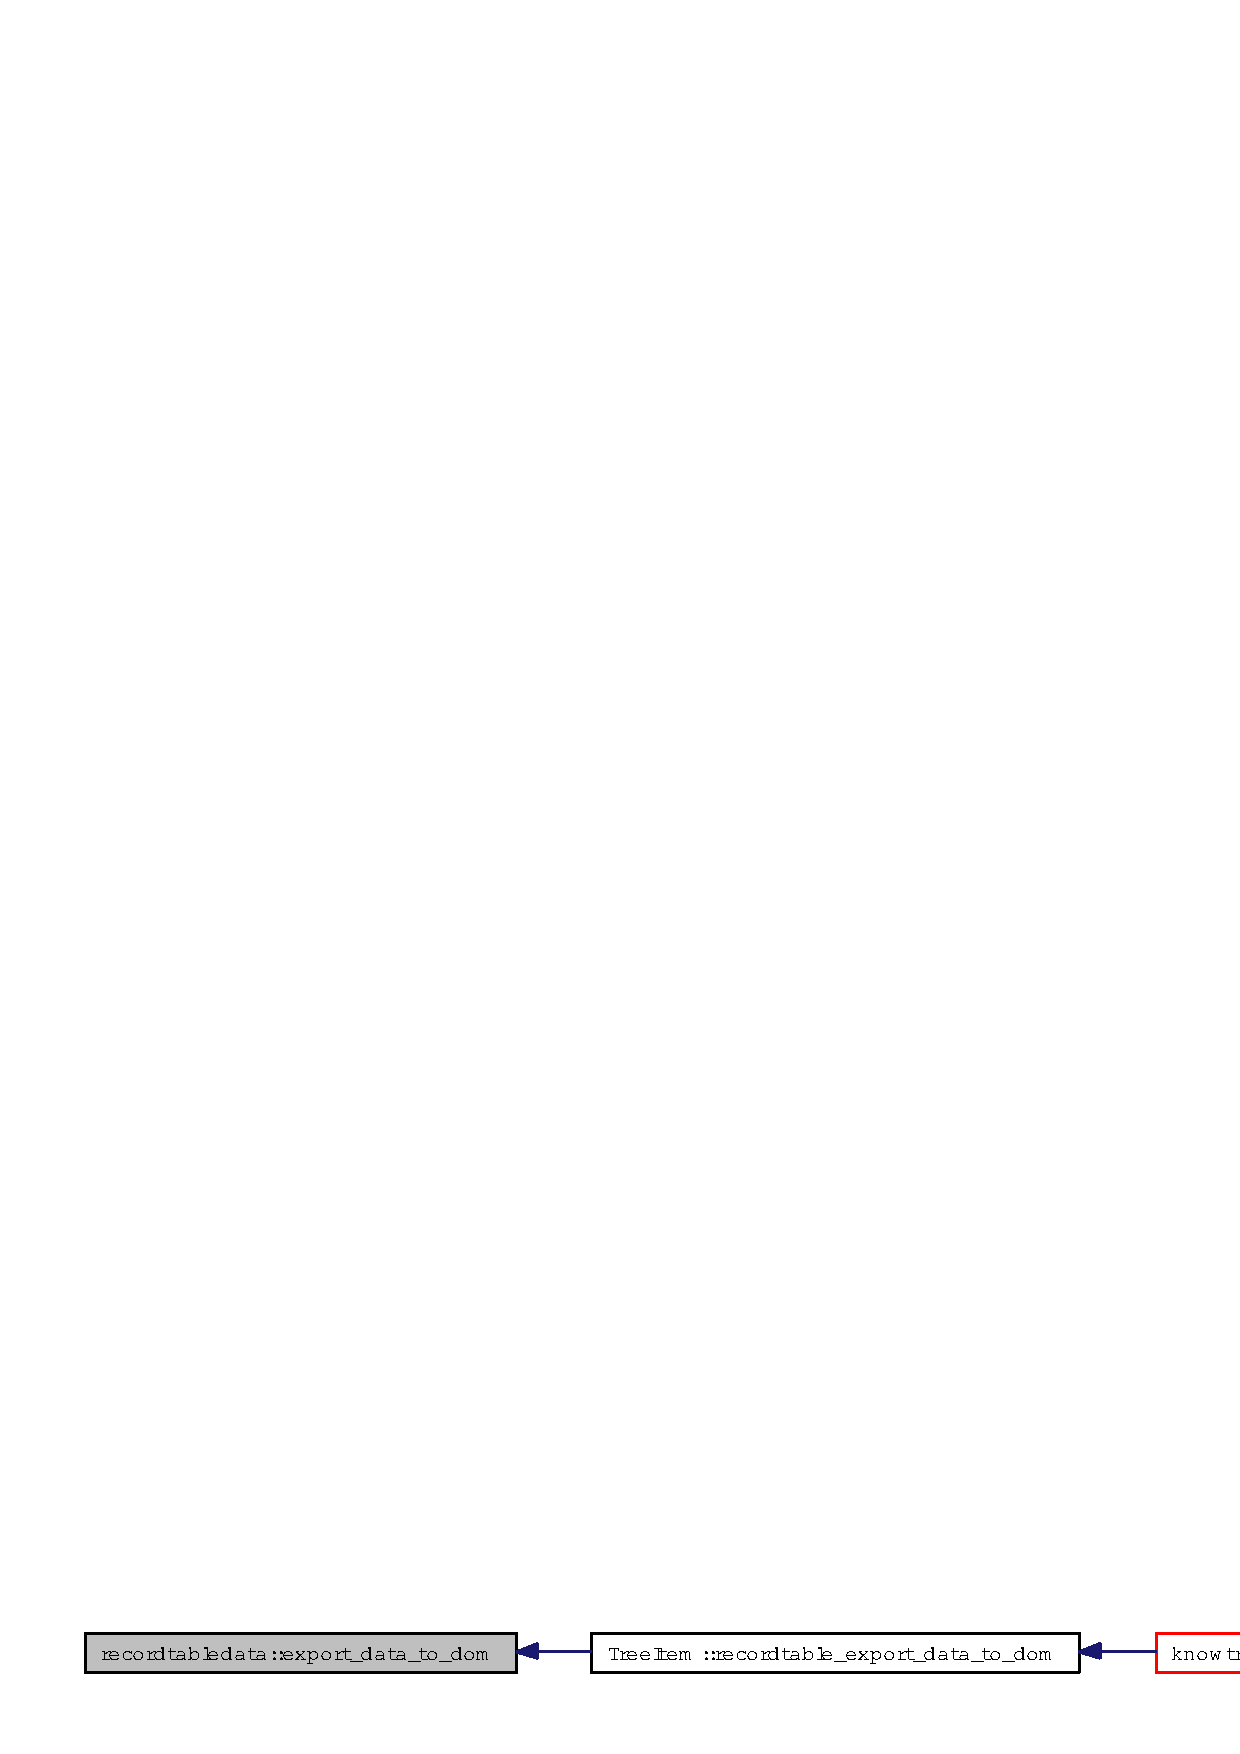
\includegraphics[width=371pt]{classrecordtabledata_fd04b0ca1500e0fd9ac3fb2d56c12b82_icgraph}
\end{center}
\end{figure}
\index{recordtabledata@{recordtabledata}!insert_new_record@{insert\_\-new\_\-record}}
\index{insert_new_record@{insert\_\-new\_\-record}!recordtabledata@{recordtabledata}}
\subsubsection{\setlength{\rightskip}{0pt plus 5cm}int recordtabledata::insert\_\-new\_\-record (int {\em mode}, int {\em pos}, QString {\em name}, QString {\em author}, QString {\em url}, QString {\em tags}, QString {\em text})}\label{classrecordtabledata_15f519acd76fc58f882e5a5d78105c61}




Definition at line 249 of file recordtabledata.cpp.

References ADD\_\-NEW\_\-RECORD\_\-AFTER, ADD\_\-NEW\_\-RECORD\_\-BEFORE, ADD\_\-NEW\_\-RECORD\_\-TO\_\-END, critical\_\-error(), appconfig::get\_\-lastidnum(), appconfig::get\_\-lastnotenum\_\-as\_\-line(), appconfig::get\_\-tetradir(), appconfig::inc\_\-lastidnum(), appconfig::inc\_\-lastnotenum(), mytetraconfig, and table.

Referenced by recordtablescreen::add\_\-new().

Here is the call graph for this function:\begin{figure}[H]
\begin{center}
\leavevmode
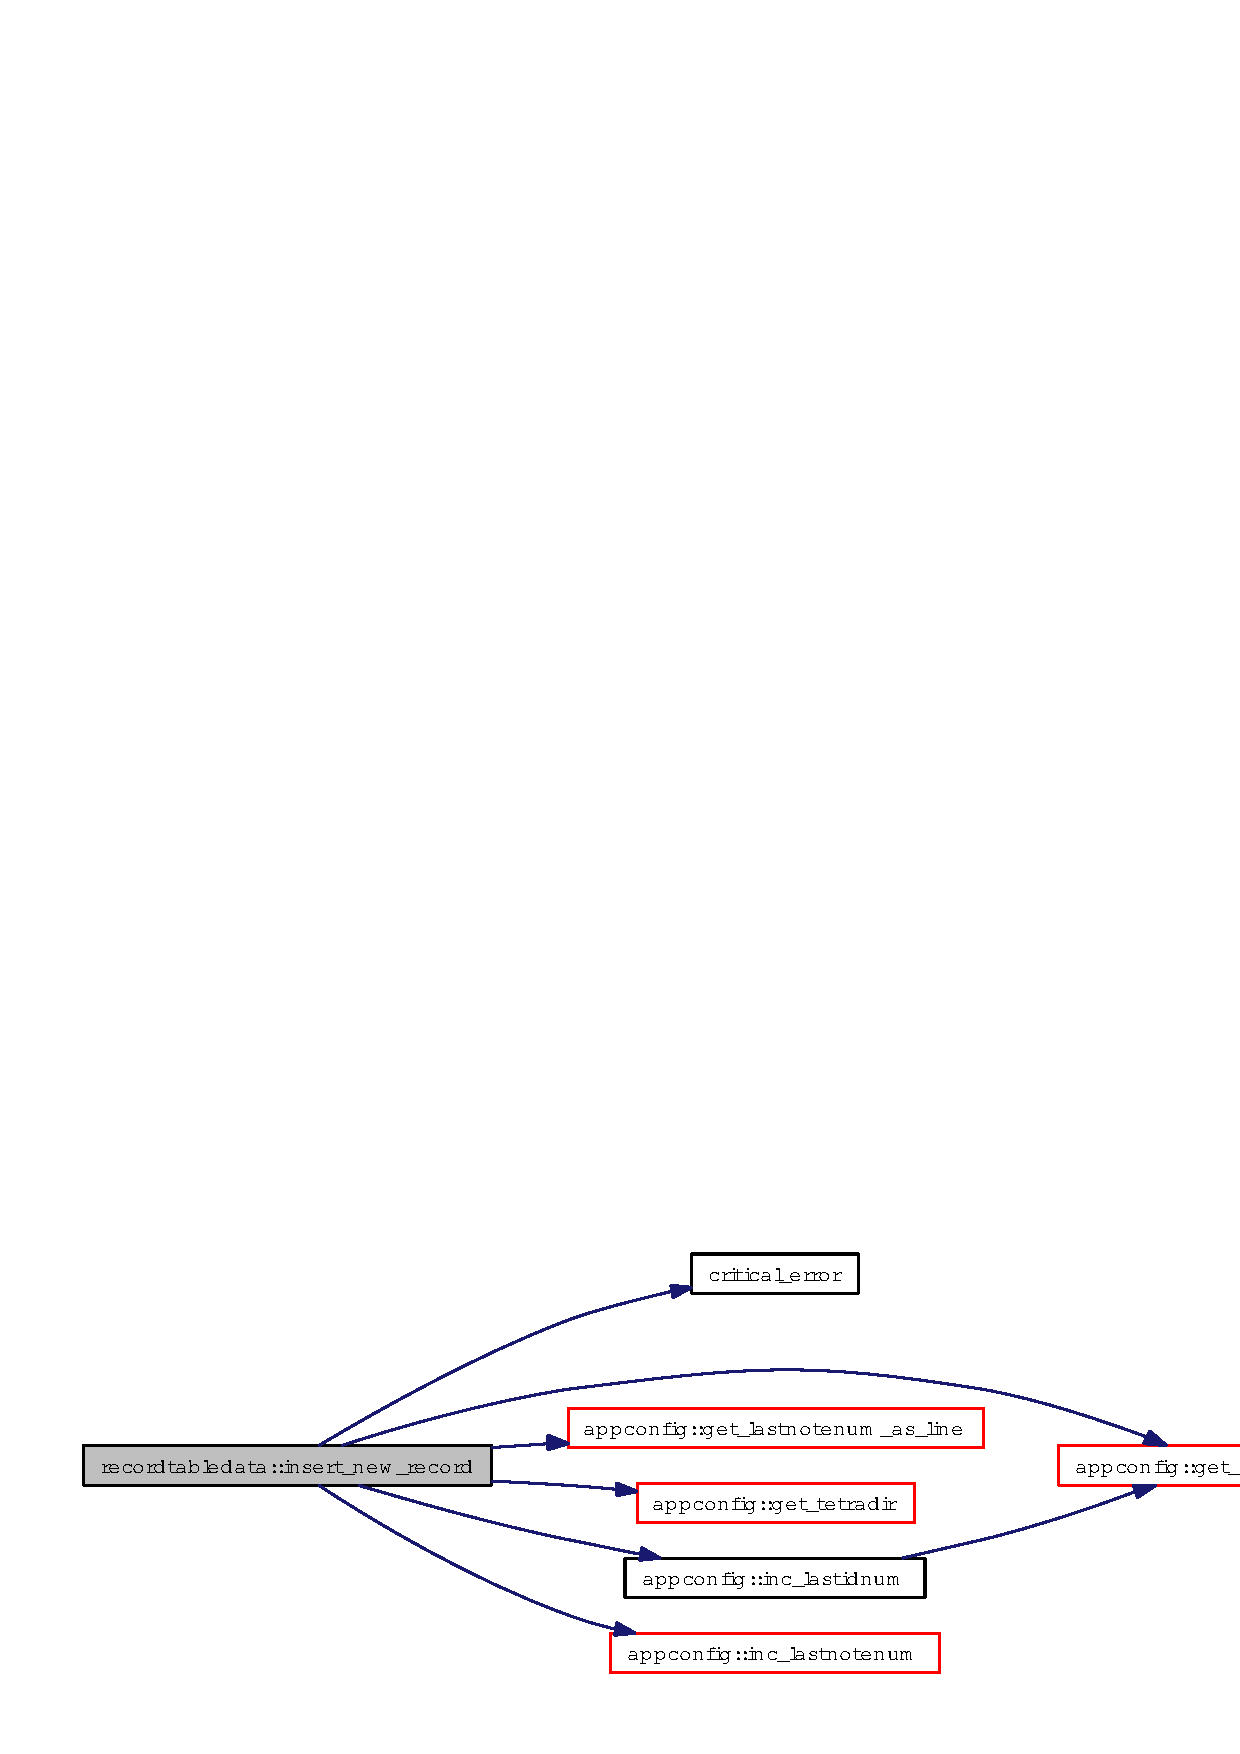
\includegraphics[width=329pt]{classrecordtabledata_15f519acd76fc58f882e5a5d78105c61_cgraph}
\end{center}
\end{figure}


Here is the caller graph for this function:\begin{figure}[H]
\begin{center}
\leavevmode
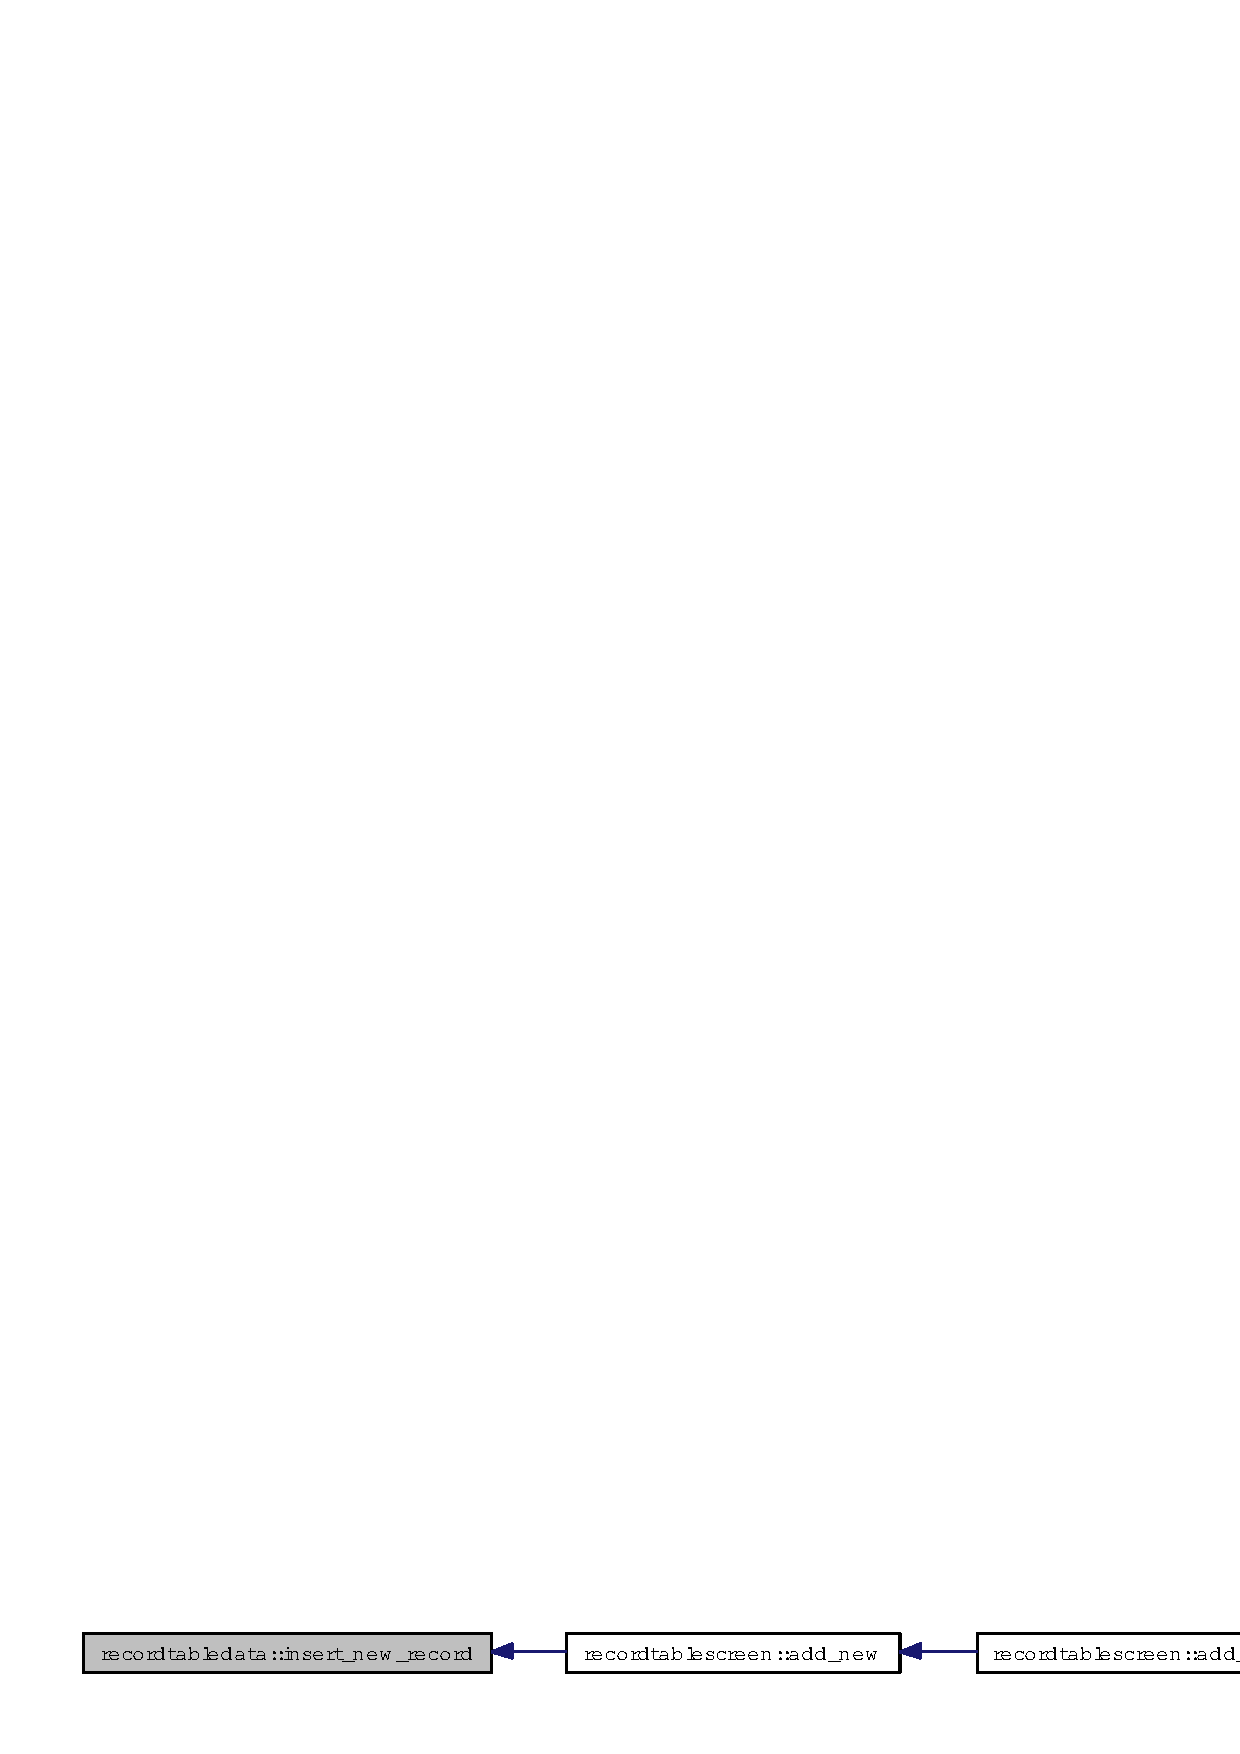
\includegraphics[width=335pt]{classrecordtabledata_15f519acd76fc58f882e5a5d78105c61_icgraph}
\end{center}
\end{figure}
\index{recordtabledata@{recordtabledata}!edit_record@{edit\_\-record}}
\index{edit_record@{edit\_\-record}!recordtabledata@{recordtabledata}}
\subsubsection{\setlength{\rightskip}{0pt plus 5cm}void recordtabledata::edit\_\-record (int {\em pos}, QString {\em name}, QString {\em author}, QString {\em url}, QString {\em tags})}\label{classrecordtabledata_437205c90b9d57a3431b1677cef71c01}




Definition at line 349 of file recordtabledata.cpp.

References table.

Referenced by recordtablescreen::edit\_\-field().

Here is the caller graph for this function:\begin{figure}[H]
\begin{center}
\leavevmode
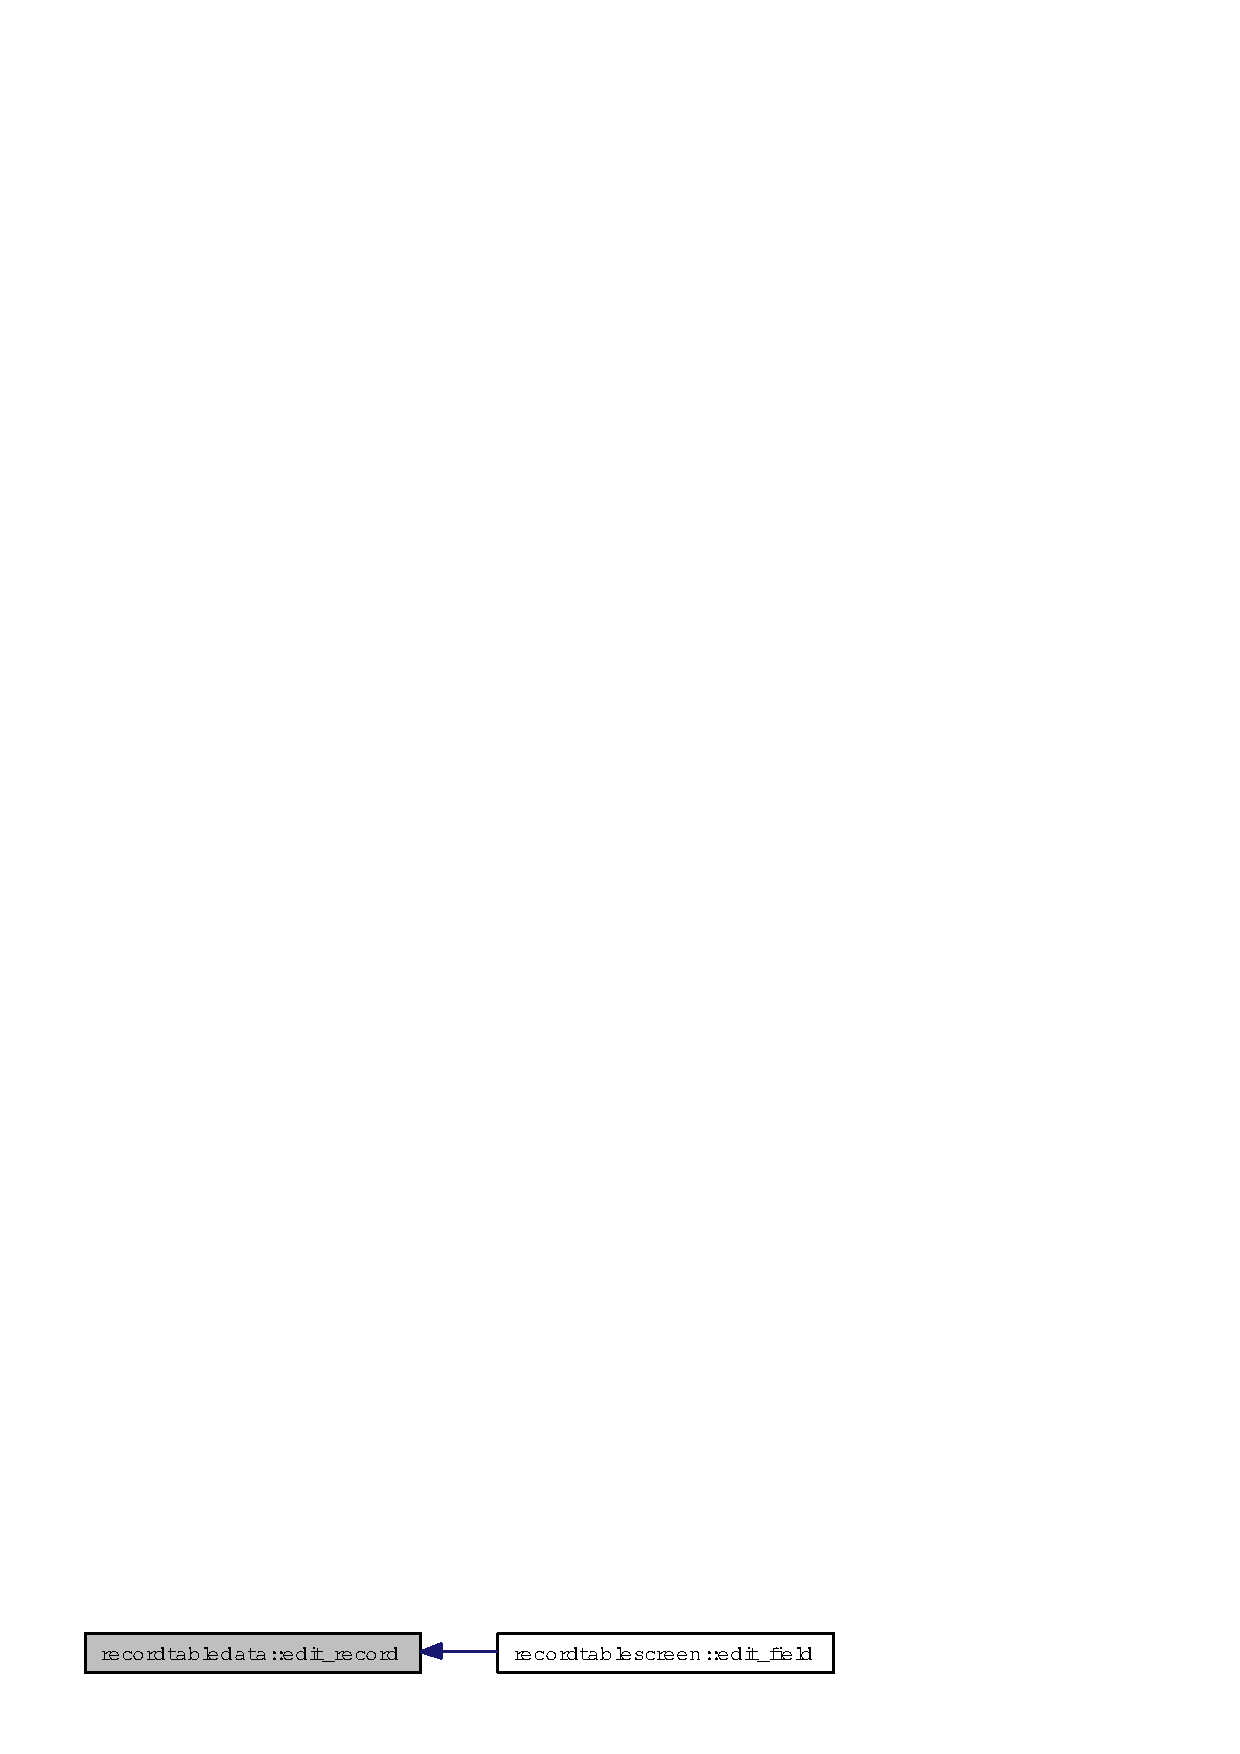
\includegraphics[width=202pt]{classrecordtabledata_437205c90b9d57a3431b1677cef71c01_icgraph}
\end{center}
\end{figure}
\index{recordtabledata@{recordtabledata}!delete_record@{delete\_\-record}}
\index{delete_record@{delete\_\-record}!recordtabledata@{recordtabledata}}
\subsubsection{\setlength{\rightskip}{0pt plus 5cm}void recordtabledata::delete\_\-record (int {\em i})}\label{classrecordtabledata_79b4a42221e3838aedc8063901fd77a3}




Definition at line 377 of file recordtabledata.cpp.

References get\_\-field(), appconfig::get\_\-tetradir(), mytetraconfig, remove\_\-dir(), and table.

Referenced by delete\_\-records().

Here is the call graph for this function:\begin{figure}[H]
\begin{center}
\leavevmode
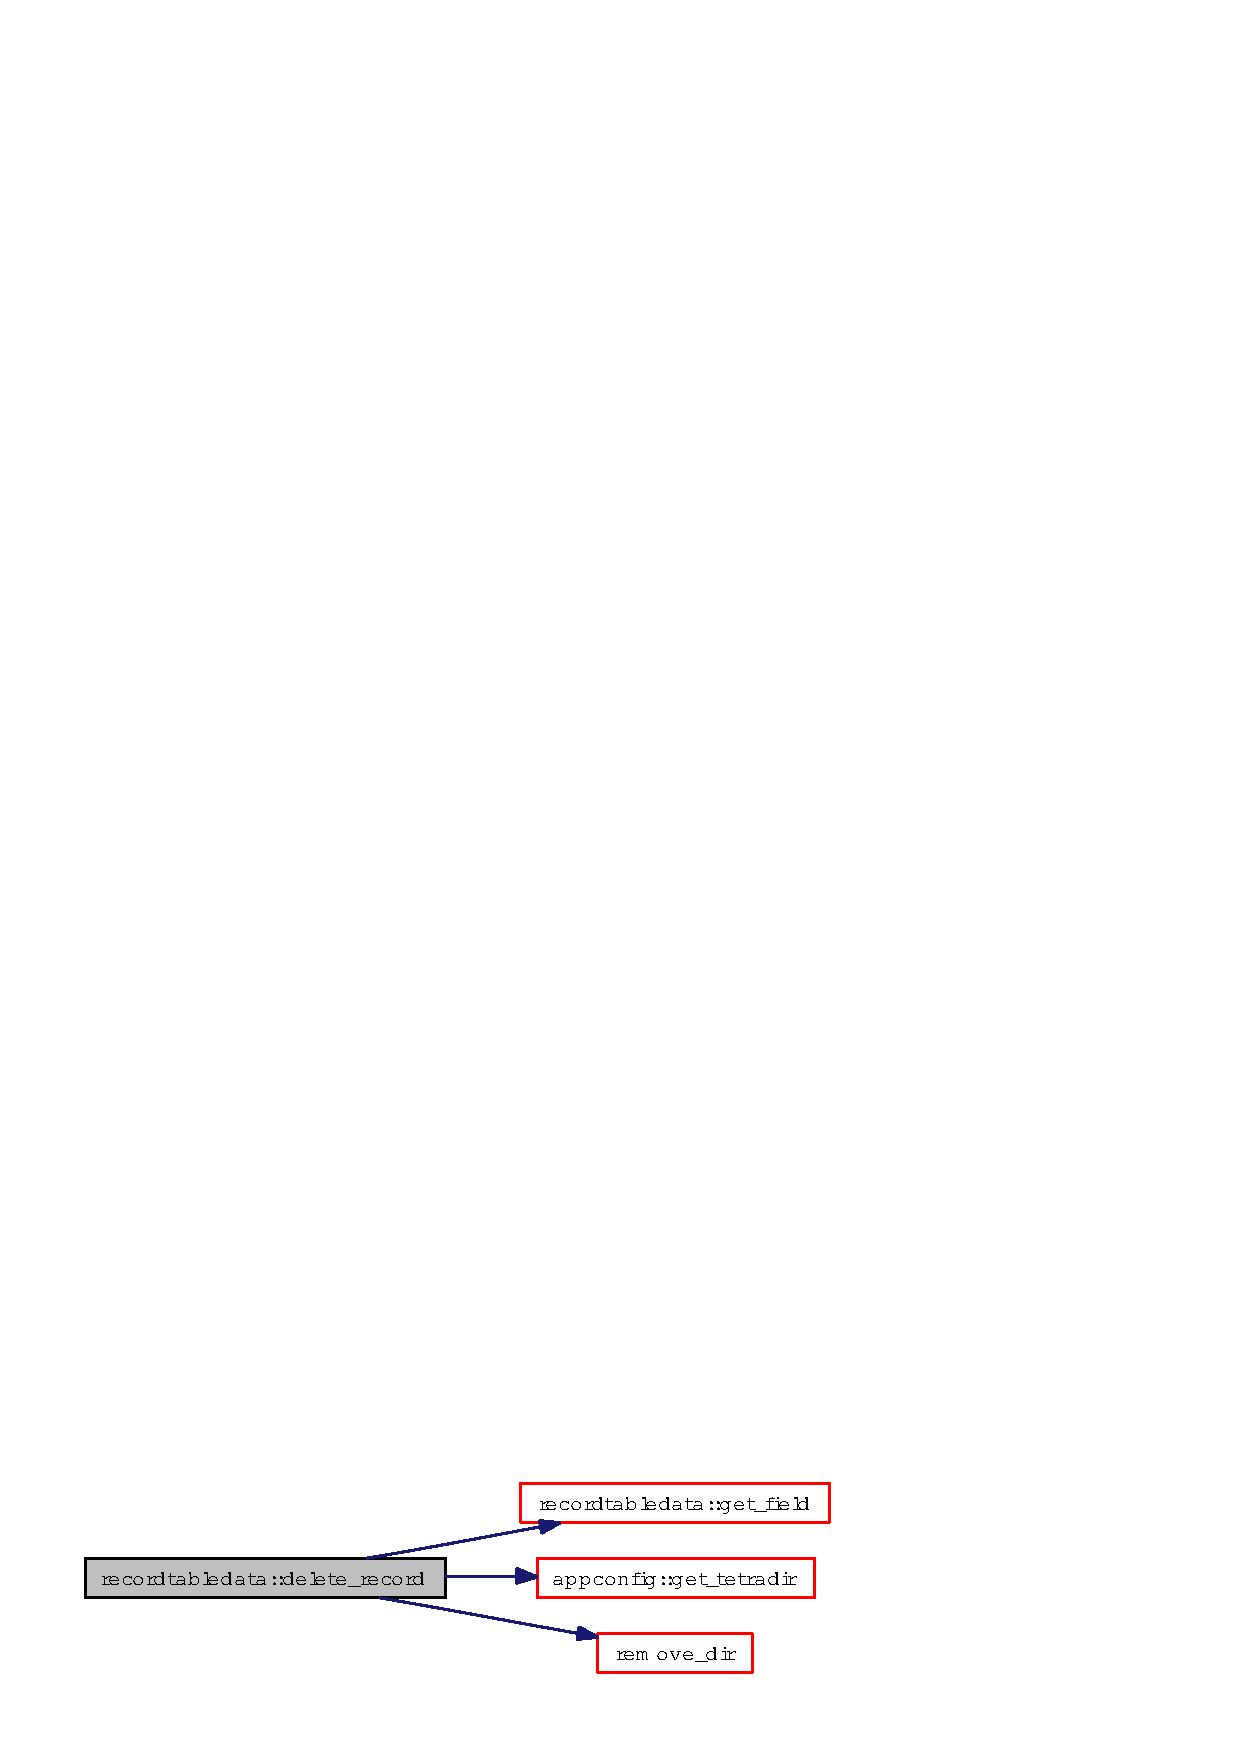
\includegraphics[width=201pt]{classrecordtabledata_79b4a42221e3838aedc8063901fd77a3_cgraph}
\end{center}
\end{figure}


Here is the caller graph for this function:\begin{figure}[H]
\begin{center}
\leavevmode
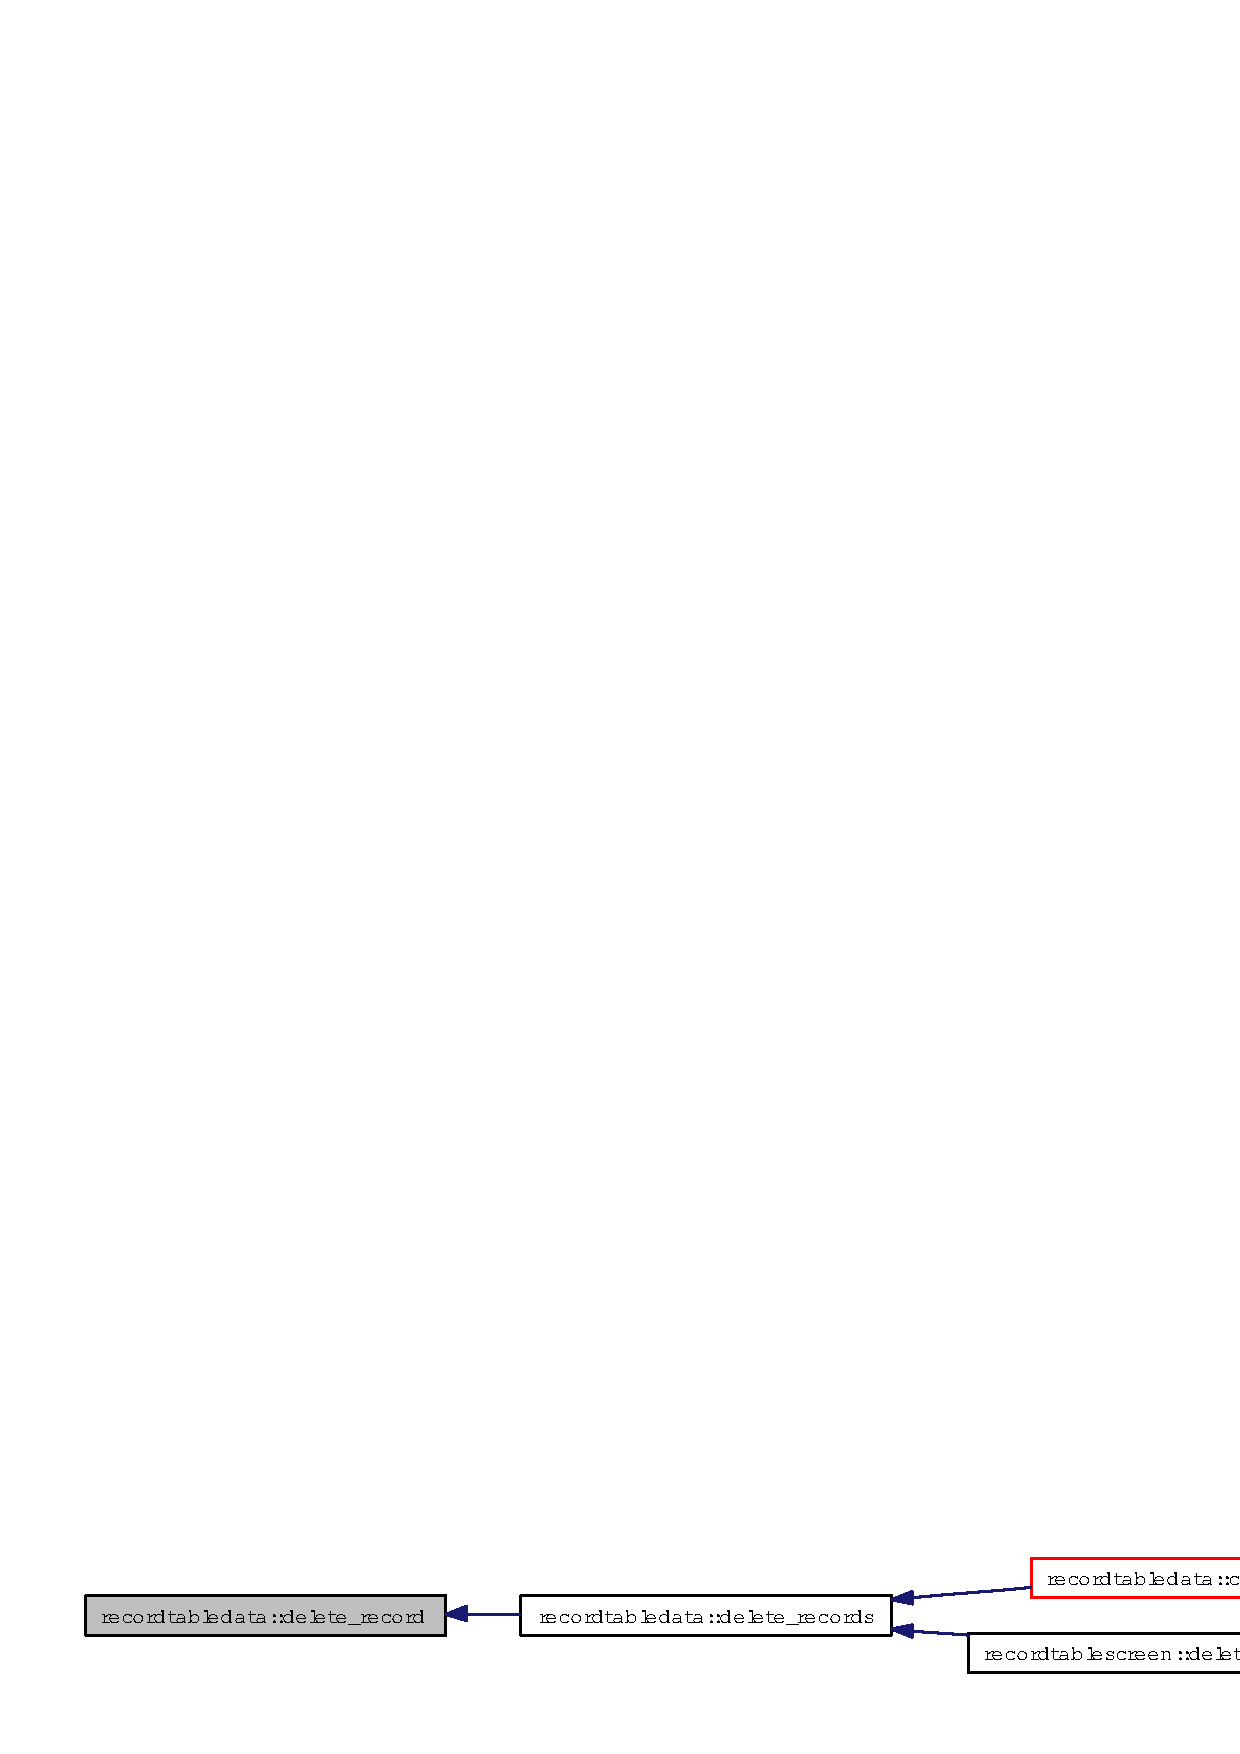
\includegraphics[width=329pt]{classrecordtabledata_79b4a42221e3838aedc8063901fd77a3_icgraph}
\end{center}
\end{figure}
\index{recordtabledata@{recordtabledata}!delete_records@{delete\_\-records}}
\index{delete_records@{delete\_\-records}!recordtabledata@{recordtabledata}}
\subsubsection{\setlength{\rightskip}{0pt plus 5cm}void recordtabledata::delete\_\-records (QVector$<$ int $>$ {\em delidx})}\label{classrecordtabledata_70252d36c2700c65a072d4c1290d2d52}




Definition at line 402 of file recordtabledata.cpp.

References delete\_\-record().

Referenced by clear(), and recordtablescreen::delete\_\-records().

Here is the call graph for this function:\begin{figure}[H]
\begin{center}
\leavevmode
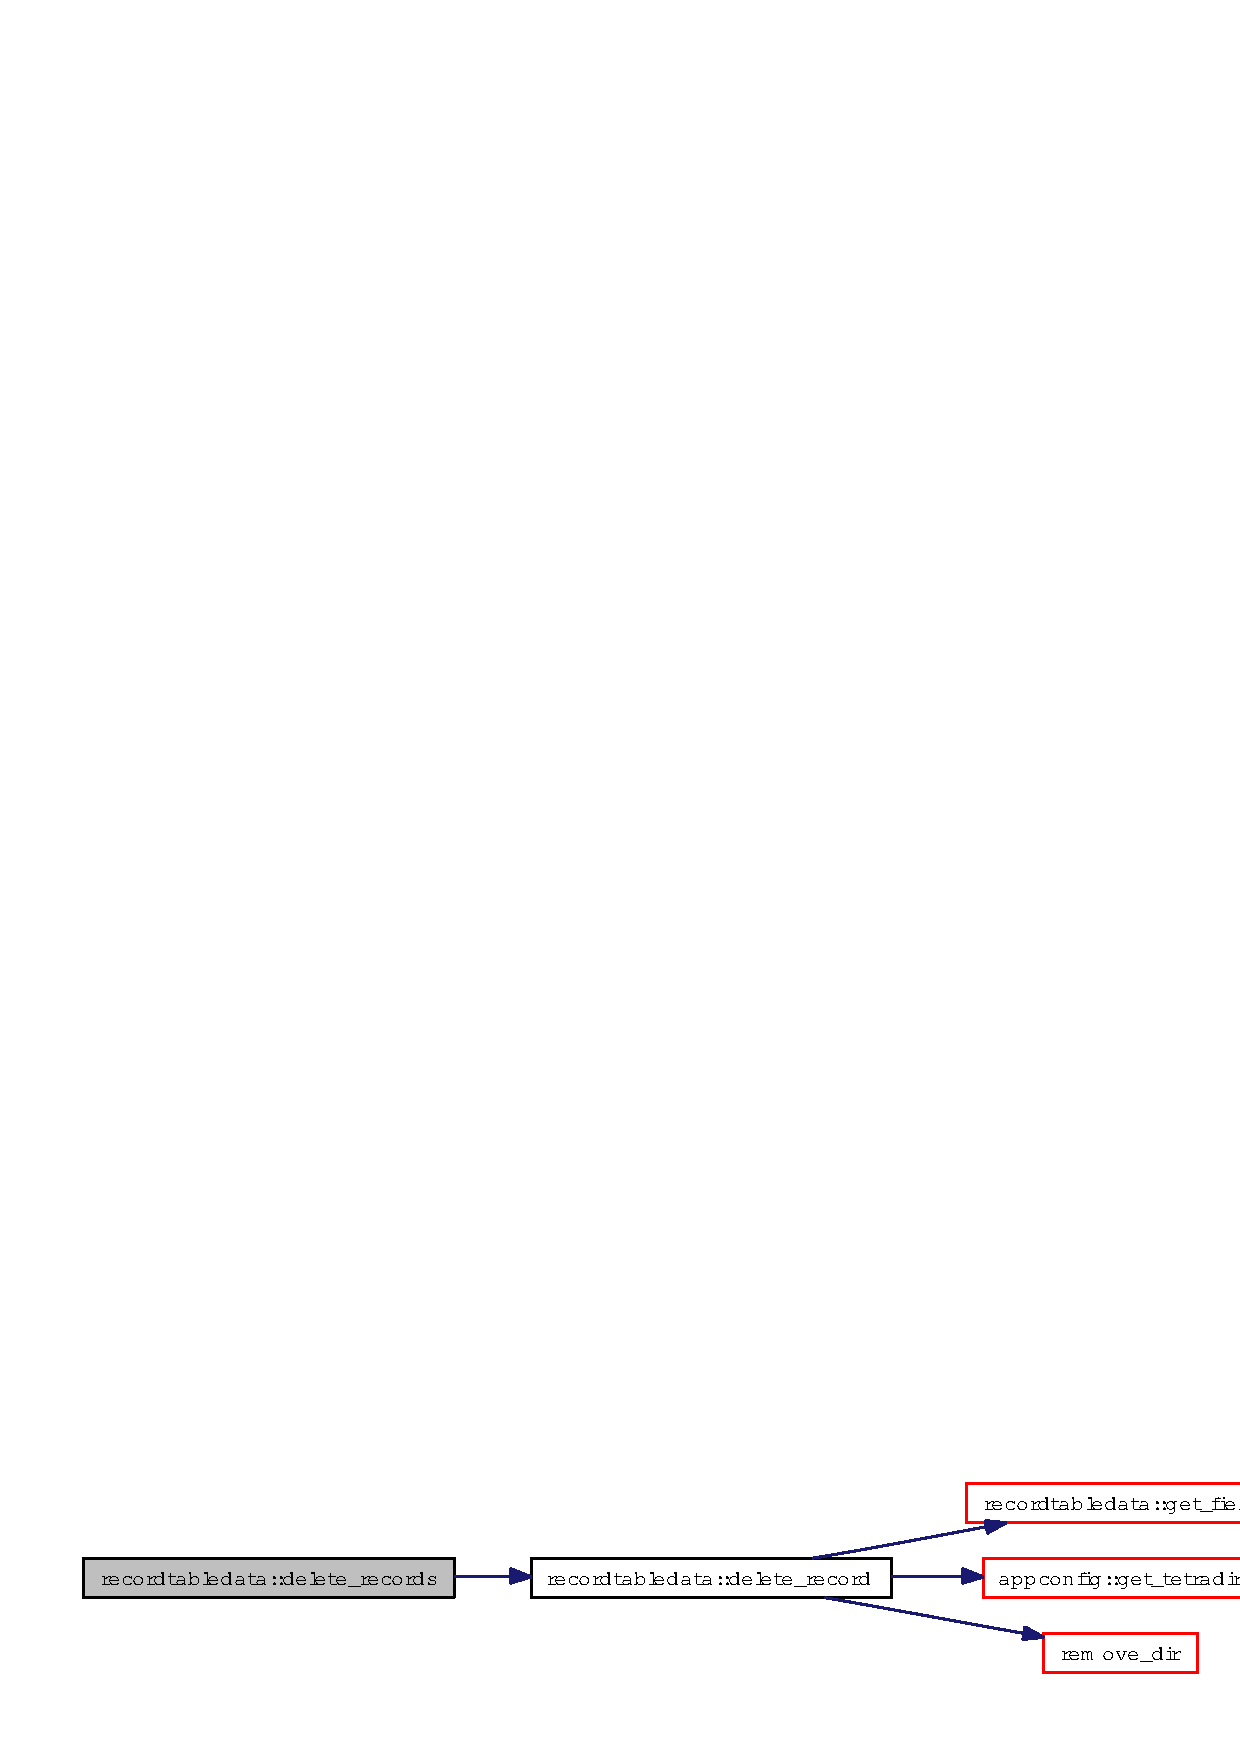
\includegraphics[width=308pt]{classrecordtabledata_70252d36c2700c65a072d4c1290d2d52_cgraph}
\end{center}
\end{figure}


Here is the caller graph for this function:\begin{figure}[H]
\begin{center}
\leavevmode
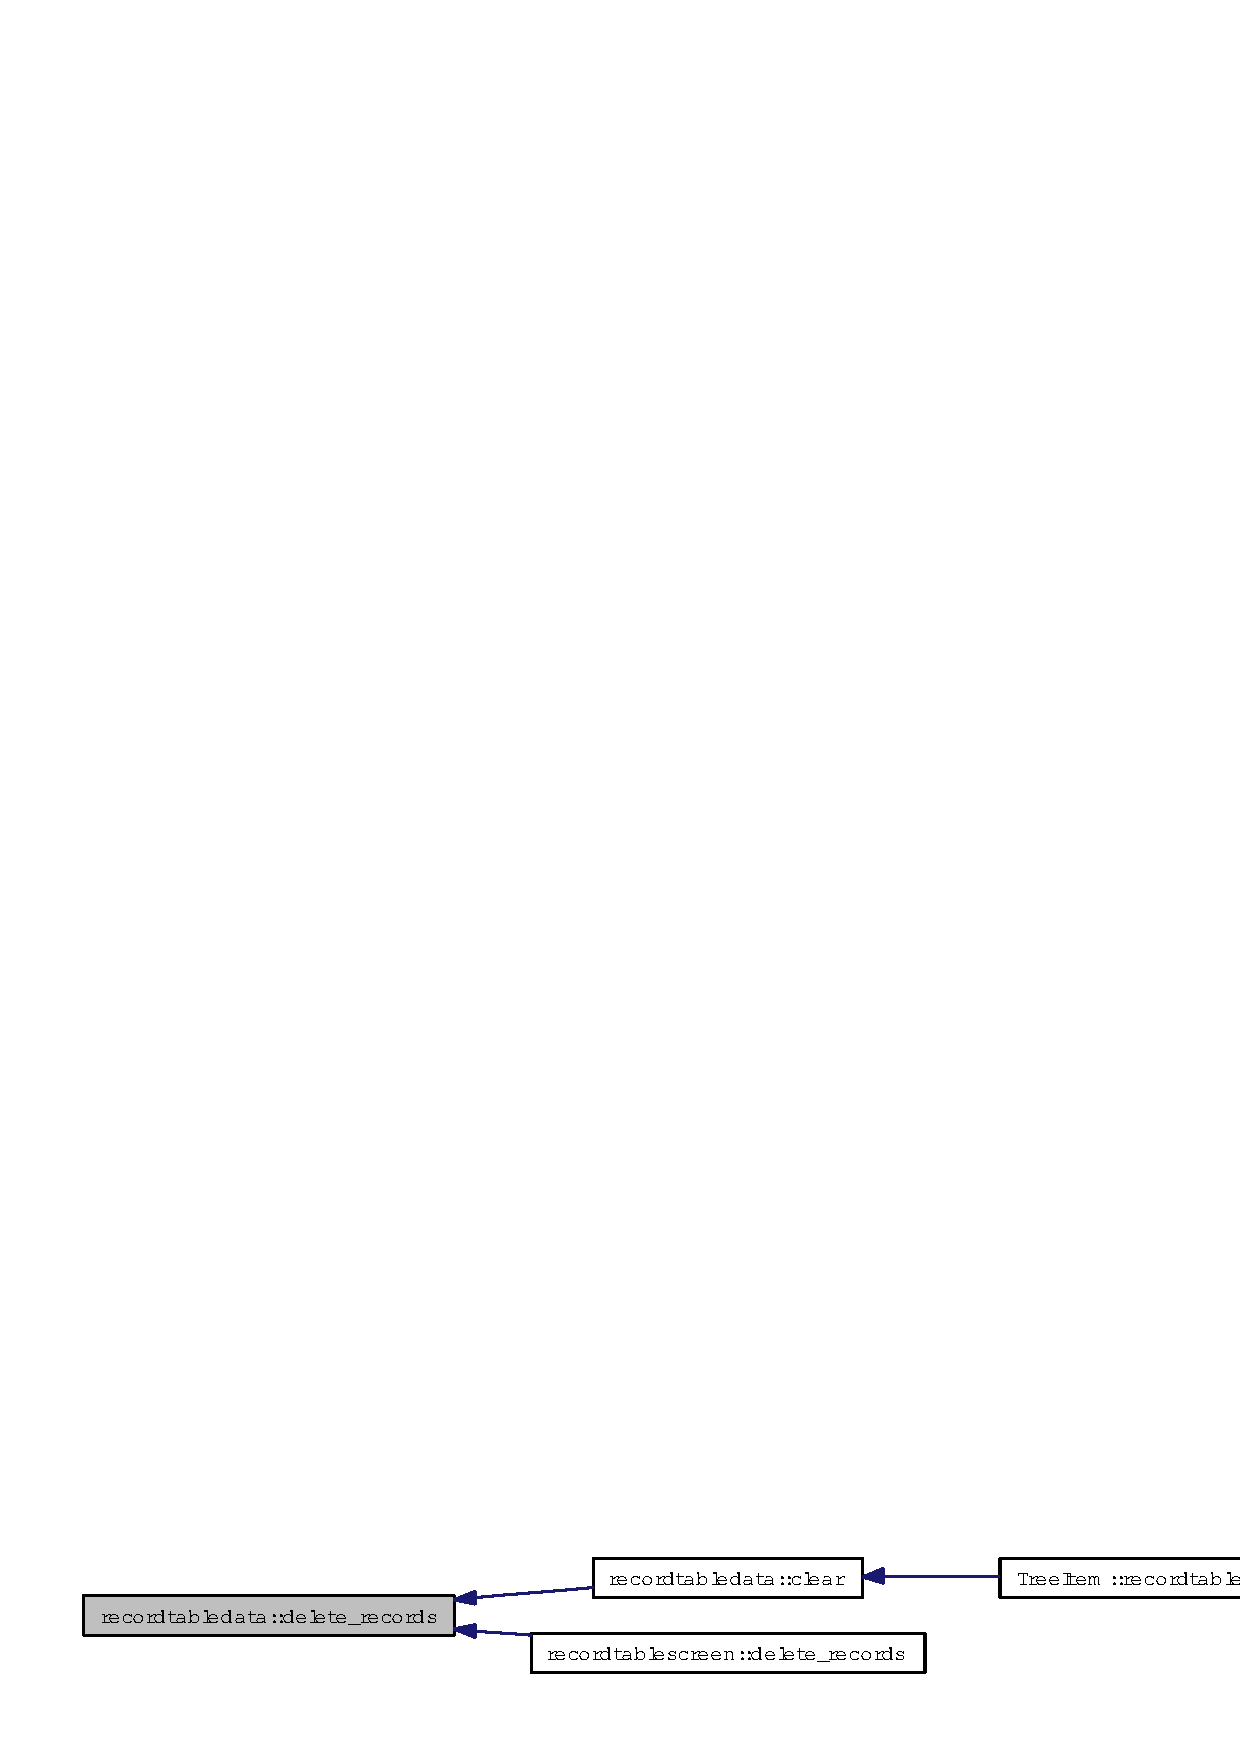
\includegraphics[width=399pt]{classrecordtabledata_70252d36c2700c65a072d4c1290d2d52_icgraph}
\end{center}
\end{figure}
\index{recordtabledata@{recordtabledata}!moveup@{moveup}}
\index{moveup@{moveup}!recordtabledata@{recordtabledata}}
\subsubsection{\setlength{\rightskip}{0pt plus 5cm}void recordtabledata::moveup (int {\em pos})}\label{classrecordtabledata_077ca508e4d7b39ff7890409650ef4d2}




Definition at line 432 of file recordtabledata.cpp.

References table.

Referenced by recordtablescreen::moveup().\index{recordtabledata@{recordtabledata}!movedn@{movedn}}
\index{movedn@{movedn}!recordtabledata@{recordtabledata}}
\subsubsection{\setlength{\rightskip}{0pt plus 5cm}void recordtabledata::movedn (int {\em pos})}\label{classrecordtabledata_ba8cc1322d315f7c7e310dff74d15053}




Definition at line 448 of file recordtabledata.cpp.

References table.

Referenced by recordtablescreen::movedn().\index{recordtabledata@{recordtabledata}!setup_data_from_dom@{setup\_\-data\_\-from\_\-dom}}
\index{setup_data_from_dom@{setup\_\-data\_\-from\_\-dom}!recordtabledata@{recordtabledata}}
\subsubsection{\setlength{\rightskip}{0pt plus 5cm}void recordtabledata::setup\_\-data\_\-from\_\-dom (QDom\-Element $\ast$ {\em dommodel})\hspace{0.3cm}{\tt  [private]}}\label{classrecordtabledata_859f66d9b583fcc73fa8011b310d4f39}




Definition at line 157 of file recordtabledata.cpp.

References table.

Referenced by init().

Here is the caller graph for this function:\begin{figure}[H]
\begin{center}
\leavevmode
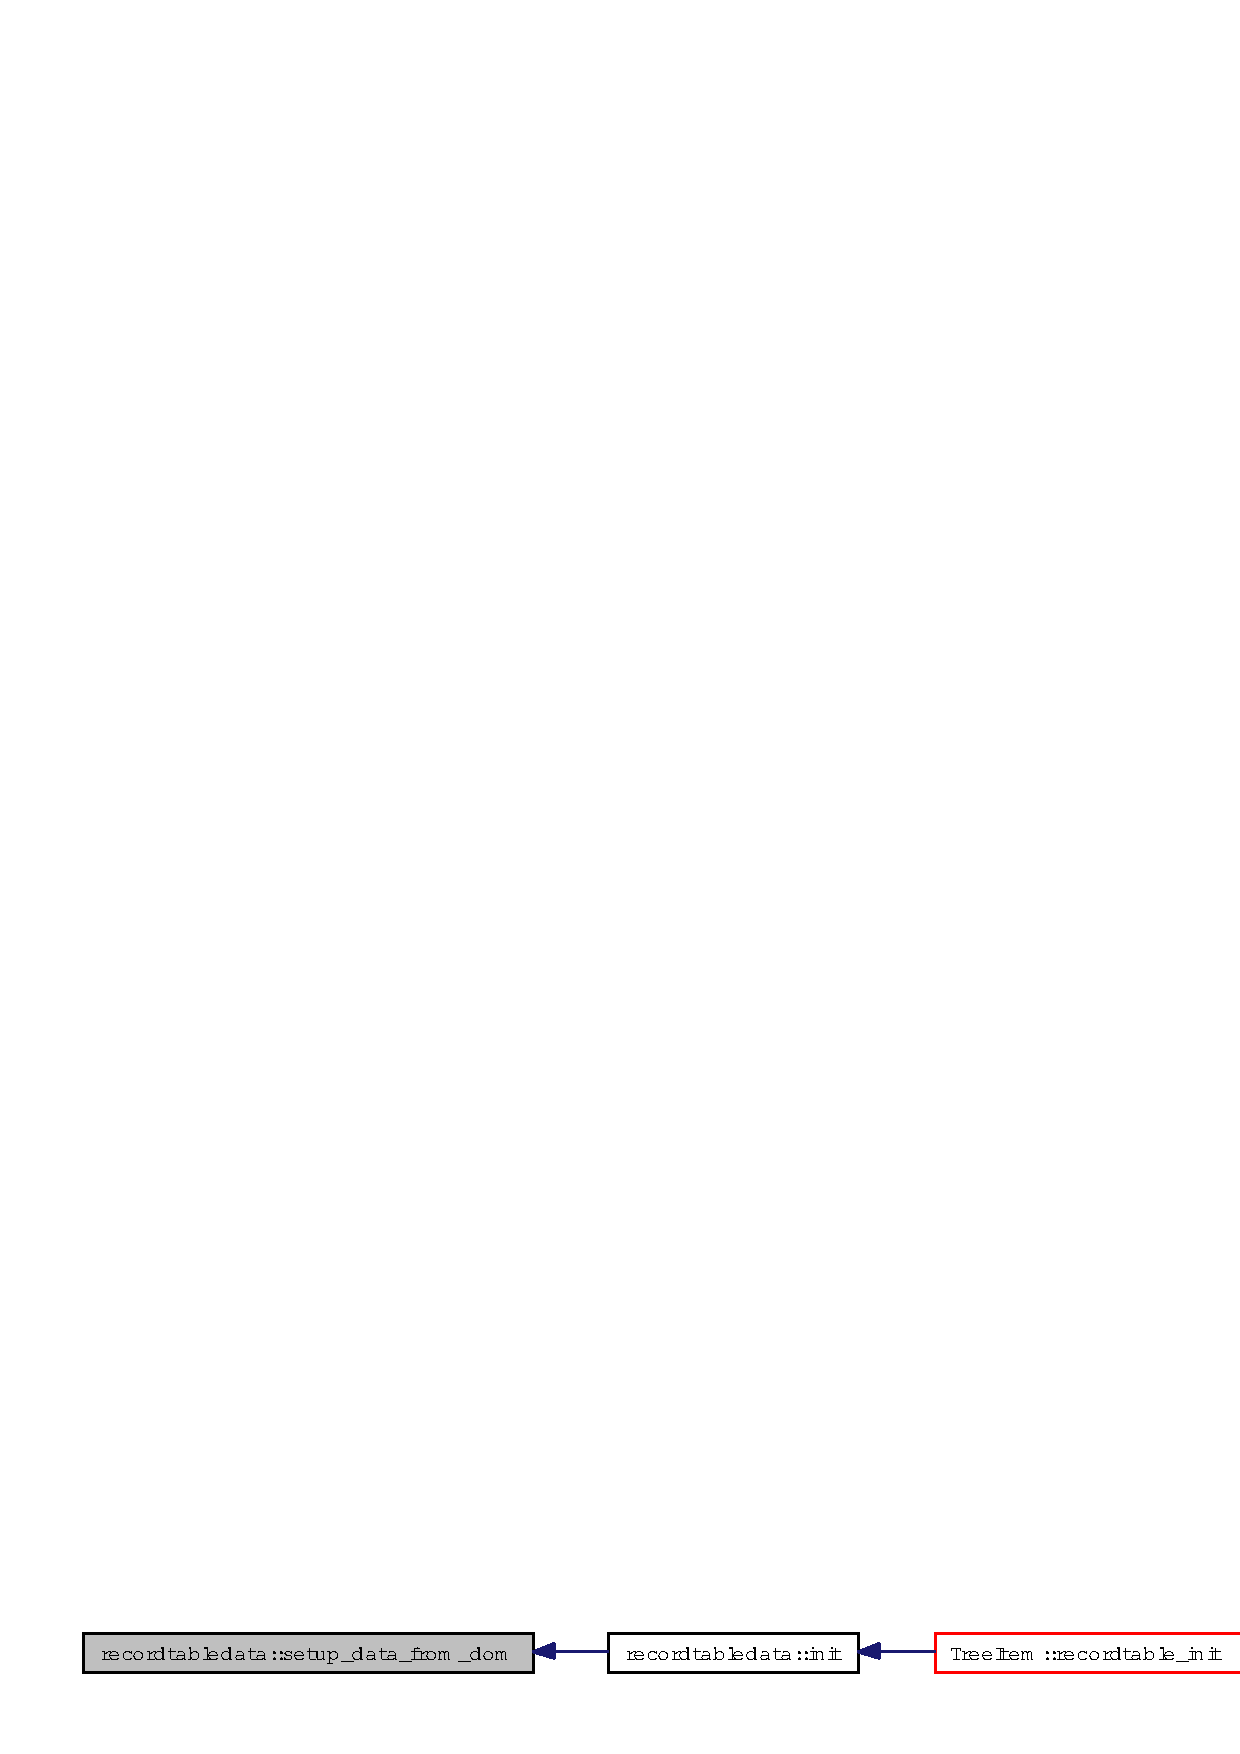
\includegraphics[width=300pt]{classrecordtabledata_859f66d9b583fcc73fa8011b310d4f39_icgraph}
\end{center}
\end{figure}


\subsection{Member Data Documentation}
\index{recordtabledata@{recordtabledata}!table@{table}}
\index{table@{table}!recordtabledata@{recordtabledata}}
\subsubsection{\setlength{\rightskip}{0pt plus 5cm}QList$<$ {\bf reclintype} $>$ {\bf recordtabledata::table}\hspace{0.3cm}{\tt  [private]}}\label{classrecordtabledata_b37a33c3cb17e1feb2d012c8008899a4}




Definition at line 68 of file recordtabledata.h.

Referenced by clear(), delete\_\-record(), edit\_\-record(), export\_\-data\_\-to\_\-dom(), get\_\-field(), get\_\-fields(), get\_\-record\_\-img(), get\_\-text(), insert\_\-new\_\-record(), movedn(), moveup(), set\_\-field(), setup\_\-data\_\-from\_\-dom(), and size().

The documentation for this class was generated from the following files:\begin{CompactItemize}
\item 
{\bf recordtabledata.h}\item 
{\bf recordtabledata.cpp}\end{CompactItemize}
